%%%%%%%%%%%%%%%%%%%%%%%%%%%%%%%%%%%%%%%%%%%%%%%%%%%%%%%%%%%
%% Congratulations, you've made an excellent choice
%% of writing your Tampere University thesis using
%% the LaTeX system. This document attempts to be
%% as complete a template as possible to let you focus
%% on the most important part: the writing itself.
%% Thus the details regarding the visual appearance
%% and even structure have already been worked out
%% for you!
%%
%% I sincerely hope you will find this template useful
%% in completing your thesis project. I've tried to
%% add comments (followed by the % sign) to clarify
%% the structure and purpose of some of the commands.
%% Most of the magic happens in the file tauthesis.cls,
%% which you are more than welcome to take a look at.
%% Just refrain from editing it in the most crucial
%% versions of the thesis!
%%
%% I wish you and your thesis project the best of luck!
%% If this template causes you trouble along the way
%% or if you've any suggestions for improving it,
%% please be in contact through GitHub
%% (<URL HERE>)
%%
%% Yours,
%%
%% Ville Koljonen
%%
%% PS. This template or its associated class file don't
%% come with a warranty. The content is provided as is,
%% without even the implied promise of fitness to the
%% mentioned purpose. You, as the author of the thesis,
%% are responsible for the entire work, including the
%% provided material. No one else is liable to you for
%% any damage inflicted on you or your thesis, were it
%% caused by using this template or not.
%%%%%%%%%%%%%%%%%%%%%%%%%%%%%%%%%%%%%%%%%%%%%%%%%%%%%%%%%%%

%%%%% NOTICE %%%%%
%% Please read through the entire template
%% (files under ./tex) to find all instructions.
%% It is possible that the attached pdf files
%% do not include the latest information.
%%%%%%%%%%%%%%%%%%

%%%%% INSTRUCTIONS FOR COMPILING THE DOCUMENT %%%%%
%% Overleaf: just click Recompile.
%% Terminal:
%%  1. pdflatex main.tex
%%  2. makeindex -s main.ist -t main.glg -o main.gls main.glo
%%  3. biber main
%%  4. pdflatex main.tex
%%  5. pdflatex main.tex
%% Similar sequence of commands is also required
%% in LaTeX specific editors.
%%%%%%%%%%%%%%%%%%%%%%%%%%%%%%%%%%%%%%%%%%%%%%%%%%%

%%% Set PDF version before doing anything else.

%%% set-pdf-version.tex
%
% This file is loaded by main.tex before any other operations, so that PDF
% version is set correctly for accessibility features.
%

\RequirePackage{ifluatex}

\def\mypdfminorversion{6}

\ifluatex

    \directlua {
        if pdf.getminorversion() \string~= \mypdfminorversion then
            if (status.pdf_gone and status.pdf_gone > 0)
            or (status.pdf_ptr and status.pdf_ptr > 0)
            then
                tex.error("PDF version cannot be changed anymore.")
            else
                pdf.setminorversion(\mypdfminorversion)
            end
        end
    }

\else

    \pdfminorversion=\mypdfminorversion

\fi


%%%%% METADATA %%%%%
%
% Always keep the following metadata up to date! This is important for your
% PDF file to comply to accessibility standards. (And yes, this information
% must remain here, before \documentclass[...]{...}.)

\def\myfititle{Värinkorjaus Splineillä}
\def\myentitle{Colour Correction using Splines}
\def\myauthor{Joni Suominen}
\def\myfithesistype{Diplomityö}
\def\myenthesistype{M.Sc Thesis}
\def\myexaminers{Professor Karen Eguiazarian \\ Researcher Vladimir Katkovnik}
\def\myfifacultyname{Informaatioteknologian ja viestinnän tiedekunta}
\def\myenfacultyname{Faculty of Information Technology and Communication Sciences}
\def\myfiprogrammename{Tietotekniikan DI-ohjelma}
\def\myenprogrammename{ Master's Programme in Information Technology}
\def\myfikeywords{Värinkorjaus, Kameran karakterisointi, Spektriherkkyys, Splini, Väritiede}
\def\myenkeywords{Colour correction, Camera characterisation, Colour science, Spectral sensitivity, Spline}
\def\mylanguagecode{en-GB}
\def\mysubject{A short description of the thesis subject.}
\def\myyear{2024}
\def\mymonth{04}
\def\myday{15}

%%%%% PREAMBLE %%%%%

%%%%% Document class declaration.
%
% The possible optional arguments are
%
%   finnish - thesis in Finnish (default)
%   english - thesis in English
%   numeric - citations in numeric style (default)
%   authoryear - citations in author-year style
%   apa - citations in APA 7 (available only in English)
%   ieee - citations in IEEE style (available only in English)
%   draft - for faster non-final works, also skips images
%           (recommended, remove in final version)
%   programs - if you wish to display code snippets
% Example: \documentclass[english, authoryear]{tauthesis}
%          thesis in English with author-year citations

\documentclass[english]{tauthesis}

%%% preamble.tex
%
% This file is for including LaTeX libraries or packages and defining your own
% commands.
%
% NOTE: The glossaries package loaded by tauthesis.cls throws a warning: No
% language module detected for 'finnish'. You can safely ignore this. All
% other warnings should be taken care of, before your thesis is submitted!

%%%%% Your packages.
%
% Before adding packages, see if they can be found in tauthesis.cls already.
% If you're not sure that you need a certain package, don't include it in the
% document! This can dramatically reduce compilation time.

% Graphs
% \usepackage{pgfplots}
%\pgfplotsset{compat=1.15}

% Subfigures and wrapping text
% \usepackage{subcaption}

%% Theorem environments and their numbering.
%
% Define both English and Finnish theorem types. These all follow the same
% counter. See the documentation of amsthm to see how these can be changed to
% suit your needs, if necessary.
%

\usepackage{amsthm}

\theoremstyle{definition}

\newtheorem{definition}{Definition}[chapter]
\newtheorem{theorem}[definition]{Theorem}
\newtheorem{lemma}[definition]{Lemma}
\newtheorem{corollary}[definition]{Corollary}
\newtheorem{example}[definition]{Example}

\newtheorem{maaritelma}[definition]{Määritelmä}
\newtheorem{lause}[definition]{Lause}
\newtheorem{apulause}[definition]{Apulause}
\newtheorem{seurauslause}[definition]{Seurauslause}
\newtheorem{esimerkki}[definition]{Esimerkki}

% Mathematics packages
\usepackage{mathtools, amssymb}
%\usepackage{bm}

% Chemistry packages
% \usepackage{chemfig}
% \usepackage[version=4]{mhchem}

% Text hyperlinking
\usepackage{hyperref}
% \hypersetup{hidelinks}

% (SI) unit handling
\usepackage{siunitx}

\sisetup{
    detect-all,
    exponent-product=\cdot,
    output-decimal-marker={,}, % for theses in FINNISH!,
    per-mode=fraction,
    fraction-function=\tfrac
}

%%%%% Your commands.

% Print verbatim LaTeX commands
\newcommand{\verbcommand}[1]{\texttt{\textbackslash #1}}

% Command for formatting code.

\newcommand\code[1]{\texttt{#1}}

% A delimiter command for the norm of a vector with mathtools.

\DeclarePairedDelimiter\norm{\lVert}{\rVert}

% Basic theorems in Finnish and in English.
% Remove [chapter] if you wish a simply
% running enumeration.
% \newtheorem{lause}{Lause}[chapter]
% \newtheorem{theorem}[lause]{Theorem}

% \newtheorem{apulause}[lause]{Apulause}
% \newtheorem{lemma}[lause]{Lemma}

% Use these versions for individually
% enumerated lemmas
% \newtheorem{apulause}{Apulause}[chapter]
% \newtheorem{lemma}{Lemma}[chapter]

% Definition style
% \theoremstyle{definition}
% \newtheorem{maaritelma}{Määritelmä}[chapter]
% \newtheorem{definition}[maaritelma]{Definition}
% examples in this style

%%%%% Glossary information.

% Use the following lines ONLY if you need more
% than one glossary. The first argument specifies
% a type label for the glossary and the second
% the displayed name.
% \newglossary*{symbs}{Symbols}
% \newglossary{label}{Displayed name}
% ...

\makeglossaries

% Use this line if using the default glossary.
% Otherwise comment out.

\loadglsentries[main]{tex/glossary.tex}

% Use this line if using more than one glossary.
% Otherwise comment out.
% \loadglsentries[symbs]{tex/sanasto2.tex}

%%%%% Citation information.

% Commonly used bibliography modifications.
% Feel free to play around with them.

%\ExecuteBibliographyOptions{%
%sorting=none,
%maxbibnames=99,
%maxcitenames=2,
%giveninits=true,
%uniquename=init,
%sortcites,
%sortlocale=fin}

%\DefineBibliographyStrings{finnish}{%
%    in = {},
%    pages = {s.},
%    page = {s.}
%}
%\DefineBibliographyStrings{english}{%
%    in = {},
%    pages = {pp.},
%    page = {p.}
%}
%
%\DeclareNameAlias{sortname}{last-first}
%\DeclareNameAlias{author}{last-first}

%\DeclareFieldFormat[%
%    article,inbook,incollection,inproceedings,
%    patent,thesis,unpublished]{citetitle}{#1\isdot}
%\DeclareFieldFormat[%
%    article,inbook,incollection,inproceedings,
%    patent,thesis,unpublished]{title}{#1\isdot}
%\DeclareFieldFormat{pagetotal}{#1 \bibstring{page}}

%\AtBeginBibliography{\renewcommand*{\makelabel}[1]{#1\hss}}

%\DefineBibliographyExtras{english}{\let\finalandcomma=\empty}

\addbibresource{tex/references.bib}
\usepackage{neuralnetwork}
\usepackage{pgfplots}
\pgfplotsset{compat=1.18}
\usepackage{bm}
\usepackage{booktabs}
\usepackage{microtype}

  \setlength\heavyrulewidth{0.20ex}
  \setlength\cmidrulewidth{0.10ex}
  \setlength\lightrulewidth{0.10ex}
\newcommand{\inputneuron}[2]{
    \ifnum #2=1
        R
    \else
        \ifnum #2=2
            G
        \else
            B
        \fi
    \fi
}

\newcommand{\outputneuron}[2]{
    \ifnum #2=1
        X
    \else
        \ifnum #2=2
            Y
        \else
            Z
        \fi
    \fi
} % You can add packages and define new commands in this file.

\begin{document}

%%%%% FRONT MATTER %%%%%

\frontmatter

%%%%% Thesis information and title page.

% Enable the use of @ character in command names.

\makeatletter

% The titles of the work. If there is no subtitle, leave the \myfisubtitle or
% \myensubtitle command arguments empty. Pass the title in the primary
% language as the first argument and its translation to the secondary language
% as the second.

\if@langenglish

    \title{\myentitle}{\myfititle}

\else

    \title{\myfititle}{\myentitle}

\fi

\if@langenglish

    \subtitle{\myensubtitle}{\myfisubtitle}

\else

    \subtitle{\myfisubtitle}{\myensubtitle}

\fi

% The author name.

\author{\myauthor}

% The examiner information. If your work has multiple examiners, replace with
%
%   \examiner[<label>]{<name> \\ <name>}
%
% where <label> is an appropriate (plural) label, e.g. Examiners or
% Tarkastajat, and <name>s are replaced by the examiner names, each on their
% separate line.

\examiner{\myexaminers}

% The finishing date of the thesis (YYYY-MM-DD).

\finishdate{\myyear}{\mymonth}{\myday}

% The type of the thesis (e.g. Kandidaatintyö or Master of Science Thesis) in
% the primary and the secondary languages of the thesis.

\if@langenglish

    \thesistype{\myenthesistype}{\myfithesistype}

\else

    \thesistype{\myfithesistype}{\myenthesistype}

\fi

% The faculty and degree programme names in the primary and the secondary
% languages of the thesis, respectively.

\if@langenglish

    \facultyname{\myenfacultyname}{\myfifacultyname}

\else

    \facultyname{\myfifacultyname}{\myenfacultyname}

\fi

\if@langenglish

    \programmename{\myenprogrammename}{\myfiprogrammename}

\else

    \programmename{\myfiprogrammename}{\myenprogrammename}

\fi

% The keywords of the thesis in the primary and the secondary languages of the
% thesis.

\if@langenglish

    \keywords{\myenkeywords}{\myfikeywords}

\else

    \keywords{\myfikeywords}{\myenkeywords}
\fi

% Make @ a regular letter again.

\makeatother

% Actually generate the title page based on the above commands.

\maketitle


%%%%% Abstracts and preface.
%
% Write the abstract(s) and the preface into a separate file for the sake of
% clarity. Pass the appropriate file name as the first argument to these
% commands. Put the \abstract in the primary language first and the
% \otherabstract in the secondary language second. Those who do not speak
% Finnish only need the first abstract. The second argument of the \preface
% command takes the place where the thesis was signed in.

\abstract{tex/abstract.tex}

\otherabstract{tex/tiivistelma.tex}

\preface{tex/alkusanat.tex}{Tampere}

%%%%% Table of contents.

\tableofcontents

%%%%% Lists of figures, tables, listings and terms.
%
% Print the lists of figures and/or tables. Uncomment either of these commands
% as required. Both are optional, but if there are many important
% figures/tables, listing them may be a good idea.

\listoffigures
% \listoftables
% \lstlistoflistings

% Misc stuff related to how the glossary is displayed. You can especially
% tweak the lengths to suit you!

\glsaddall
\setglossarystyle{taulong}
\setlength{\glsnamewidth}{0.25\textwidth}
\setlength{\glsdescwidth}{0.75\textwidth}
\renewcommand*{\glsgroupskip}{}

% Print the default glossary of abbreviations, if necessary. Otherwise comment
% out. The appropriate Finnish variant is 'Lyhenteet'

\printglossary[title={Glossary}]

% Print more than one glossary with these lines. Otherwise comment out.

% \printglossary[type=symbs]
% \printglossary[type=label]
% ...

%%%%% MAIN MATTER %%%%%

\mainmatter

% Write each of the chapters of the thesis into a separate file for the sake
% of clarity. They can be \input as shown below. Give both the chapters and
% their files as descriptive names as possible.

\chapter{Introduction}%
\label{ch:introduction}

Digital cameras have become indispensable tools in today's society, playing pivotal roles across scientific research, industrial applications, and consumer needs. However, their spectral sensitivities differ markedly from the human visual system, leading to discrepancies in color representation and interpretation. Such deviations not only impact aesthetic quality but also significantly affect the accuracy of data-dependent applications, such as computer vision, medical imaging, and remote sensing. 

To view the colours of the image as if a human had viewed the scene, color correction has to be performed in order to map the colors from the camera's color space to a reference color space related to the HVS.



\chapter{Human Visual System}%
\label{ch:hvs}

To produce colour images of a scene on a digital camera that resembles how a human might perceive it, it is important to understand how the human visual system functions. A cross-section of the human eye is shown in \ref{fig:humaneye}. Many parts of the human eye have direct correspondences in a typical digital camera, such as the lens (and cornea) which focuses an inverted image onto the retina, similar to how a lens in a digital camera focuses the image to a sensor. The ciliary muscles attached to the lens can also change its shape, when focusing at different distances is required, much like how camera lenses with variable focal length work. The pupil and iris together create a system that is comparable to the adjustable aperture of a digital camera, controlling the amount of light that enters the eye.

\begin{figure}
    \centering
    \pdftooltip{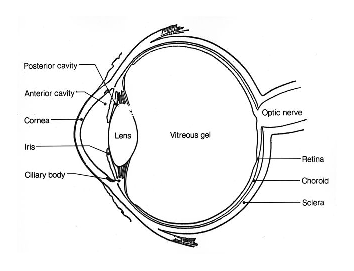
\includegraphics[width=0.7\textwidth]{figures/eye.eps}}{lol}
    \caption{Cross-section of the human eye \cite{humaneye}}
    \label{fig:humaneye}
\end{figure}

\section{Retinal receptors}

At its core, the retina of the human eye consists of receptors of different, which can be divided into two subtypes, rods and cones. The former operates primarily during dim light conditions, when the human vision is said to be scotopic, while the latter operates during well lit conditions.


The rods activate during low-light conditions, such as under moonlight, providing us monochromatic "night vision", more commonly referred to as the scotopic vision. On the contrary, the cones operate during well-lit conditions, such as daylight, allowing us to perceive colours while the photopic vision system is active. The reason why colours are perceivable during photopic vision and not scotopic vision is, that there are three types of cones, each sensitive to different range of visible wavelengths, while there is only one a single cone type.  \cite[4-5]{measuringcolour}

On the boundaries of these two conditions, known as the mesopic vision, both the rods and cones are active, which results in a phenomenon where colours are visible but they appear darker and blue-ish. This is known as the Purkinje effect. \cite[5]{measuringcolour}

\section{Spectral responsivity}

% Although Newton, using a prism, had already discovered in the 17th century that white light is a combination of several color components of different wavelengths, it was not until centuries later, that the trichromatic theory was proposed by Young. The theory suggested that the human eye consists of three receptors, sensitive to red, green and blue wavelengths respectively, and all colours could be produced by a mixture of them. Experiments during the 20th century have proven this to be partially correct, as there are three types of color receptors that form the primary response to those exact colours, but they also respond to larger range of colors. \cite{colorimetry}

% Various other theories were also proposed in addition to the trichromatic theory, such as the opponent-color theory, and produced results that were supported by empiric results and could explain certain phenomena \cite{colorimetry}. Robust test scenarios were designed during the 20th century to measure the relative responsiveness of cones and rods. By evaluating the relative responses at a densely sampled interval, spectral responsivity curves are obtained. \cite{measuringcolour} Readers interested in details of these measurements can be referred to chapters 1 and 2 in \cite{measuringcolour} and chapters 1-3 in \cite{colorimetry}.

To be able to model the human eye computationally, such as in digital cameras, its important to quantify how sensitive the eye is at some wavelength relative to some other wavelength. A standard was published in 1931 consisting of data collected by Wright and Guild from psychovisual experiments on subjects with standard vision under photopic vision. The subjects were asked to match a reference light, at some known wavelength, using a combination of three different lights with wavelengths of 435.8, 546.1 and 700 nm, corresponding roughly to the blue, green and red wavelengths respectively. \cite{wrightetguild}

These results from the two observers were combined and standardized by CIE (Commission internationale de l'éclairage), an international commission on illumination \cite{CIE}. The so called CIE 1931 RGB color matching functions are shown in figure \ref{fig:rgb}, which denote the amount of each color to match the reference light. The choice of three primaries posed some problems, as its not possible to match every color with three primaries, and thus for example red is negative in the range of 450-550 nm, as some of it had to be added to the reference light instead of the to the combination of two other primaries. \cite{measuringcolour}

To simplify computations and to make the model more interpretative, at the same time in 1931 introduced another set of color matching functions based on the previous, but with an idea that all the functions should be strictly positive, and one of them should correspond to the luminance of the color. Thus another, much more widely used, set of functions called the CIE 1931 XYZ color matching functions, was published. The functions are shown in figure \ref{fig:xyz}.


%The entity responsible for standardizing the results of these measurements is CIE (Commission internationale de l'éclairage) \cite{CIE}. They have released several standardized spectral responsivity curves, such as the spectral luminous efficiency function under scotopic vision for the standard observer in 1924, and similary for photopic vision in 1955 \cite{observer}. These measure the relative brightness across the visible wavelength range, and have been computed as the average of multiple observers with normal vision.

%In 1931, CIE published perhaps its most important standard for the colour industry, namely the 1931 CIE colour matching functions (CMFs), based on measurements by Wright and Guild. These define the relative amounts of the three colour primaries Red (700 nm), Green (546.1 nm) and Blue (435.8 nm) that are required to reproduce every colour in the visible range.\cite{measuringcolour} The function is seen in figure \ref{fig:rgb}.

\begin{figure}
    \centering
    \pdftooltip{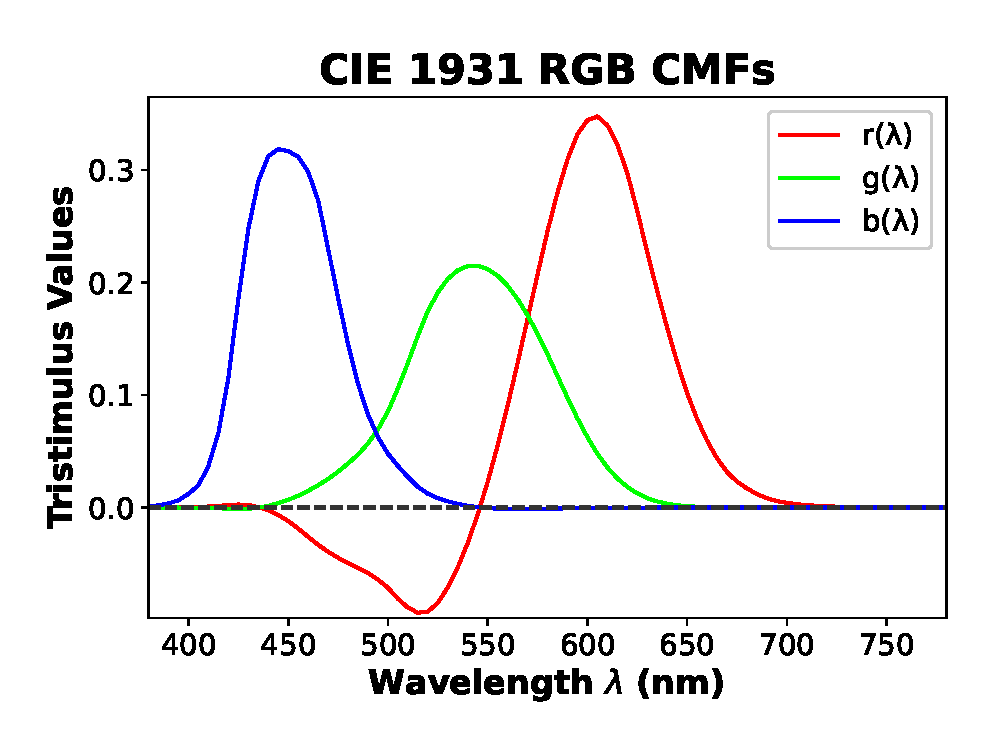
\includegraphics[width=\textwidth]{figures/cie_rgb.eps}}{CIE RGB CMFs}
    \caption{CIE RGB  \cite{humaneye}}
    \label{fig:rgb}
\end{figure}

\begin{figure}
    \centering
    \pdftooltip{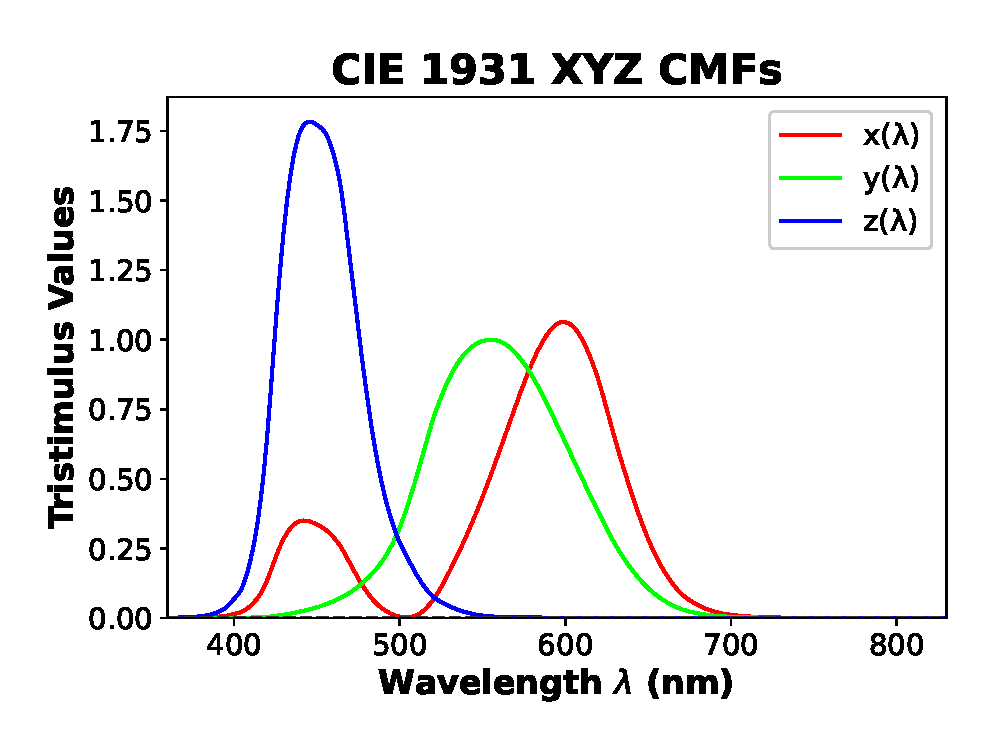
\includegraphics[width=\textwidth]{figures/cie_xyz.eps}}{CIE XYZ CMFs}
    \caption{CIE XYZ  \cite{humaneye}}
    \label{fig:xyz}
\end{figure}

\section{Tristimulus values}

From the spectral sensitivities shown in figures \ref{fig:rgb} and \ref{fig:xyz}, its possible to compute the so called tristimulus values, which mathematically describe the response of the eye to to the light that reaches the retina. The responses are computed by integrating the product of the illuminant's power spectral distribution, spectral reflectance of the object and the spectral responsivity of the sensor for given colour.

As one of the components, Y, corresponds to the luminance of the color, it makes sense to normalize it between 0 and 100 to treat is a percentage. The normalization factor $k$ can be computed as the response of the Y channel to light reflected from a perfectly white surface with Lambertian reflectance as follows

\begin{equation}
\label{eq:normalization}
 k = \frac{100}{\int_{380}^{780} E(\lambda) S_Y(\lambda) \, d\lambda},
\end{equation}

where $100$ is a scaling factor, $E(\lambda)$ is the spectral power distribution of a given illuminant, and $S_Y(\lambda)$ is the cone sensitivity for Y \cite{rowlands2020physics}. Note, that $1$ is often used as the scaling factor in numerical computation for simplicity.

The tristimulus value $T$ corresponding to either $X$, $Y$ or $Z$ is then given by

\begin{equation}
\label{eq:tristimulus}
T = k \int_{380}^{780} E(\lambda) R(\lambda) S_T(\lambda) \, d\lambda,
\end{equation}

where $E(\lambda)$ is the spectral power distribution (SPD) of the illuminant, $R(\lambda)$ is the spectral reflectance of the object, and $S_T(\lambda)$ is the sensitivity of the cones for tristimulus value \( T \) (either \( X, Y, \) or \( Z \)).

\begin{figure}
\centering
\scalebox{1.5}{%
\begin{tikzpicture}
  
  % Set the bounding box manually for more space at the bottom

  % Illuminant
  \draw[fill=yellow] (2,3) circle [radius=0.2] node[above=5pt] {Illuminant};
  \draw[->, ultra thick, yellow] (1.9,2.8) -- (1,1);

  % Surface
  \draw[fill=blue!40] (0.8,1.5) rectangle (1,0.5) node[midway, yshift=0.7cm] {Surface};

  % Sensor/Eye
  \draw[fill=red!40] (3,1.5) rectangle (3.2,0.5) node[midway, yshift=0.7cm] {Sensor/Eye};
  \draw[->, ultra thick, orange] (1,1) -- (3,1);

  % Annotations without lines
  \node[font=\small] at (0.5,2.5) {Incident Light};
  \node[font=\small] at (2,0.2) {Reflected Light};

\end{tikzpicture}
}


\caption{Light to eye model}
\label{fig:light}
\end{figure}

\section{Chromatic Adaptation}
\label{sec:chromaticadaptation}
Although one would assume that the tristimulus system is enough to model the human visual system, the human eye has the ability to adapt these sensitivities under different illuminant conditions. Even though the same scene under two different illuminants will produce distinct tristimulus values, the human visual system will perceive the colours the same. For example, a white sheet of paper will look white under sunlight and fluorescent light source. This feature is called chromatic adaptation. \cite[146-149]{fairchild}

Lots of research has addressed this phenomena during the past century, and the current ideas are only approximations of the complex biological process. The most common and oldest hypothesis was proposed by Johannes von Kries in 1902, where he suggested that the human visual system adapts to changing illumination by applying gain multipliers to the cone sensitivities. \cite[168-171]{fairchild} This effectively results in a set of coefficients for each illuminant, and can be mathematically formulated as follows

\begin{equation}
\begin{bmatrix}
L' \\
M' \\
S' \\
\end{bmatrix}
=
\begin{bmatrix}
1/k_L & 0 & 0 \\
0 & 1/k_M & 0 \\
0 & 0 & 1/k_S \\
\end{bmatrix}
\begin{bmatrix}
L \\
M \\
S \\
\end{bmatrix}
,
\end{equation}

where $L$, $M$, $S$ are the responses of the Long, Medium and Short wavelength cones to the original light source, $L'$, $M'$, $S'$ are the transformed responses after adaptation, and $k_L$, $k_M$, $k_S$ are the von Kries coefficients. The can be computed by substituting the Y channel sensitivity with cone sensitivities in formula \ref{eq:normalization}, using an appropriate scaling factor instead of $100$. This formula effectively removes effect of the illuminant and ensures that neutral objects have the same response under every light source.

Even in his publication, von Kries argued that his proposal was a gross oversimplification, but in practice, the method is still applied and it has been proved to be a good approximate \cite[170-171]{fairchild}. For example, consumer digital cameras often follow this model when simulating chromatic adaptation. More sophisticated models of chromatic adaptation exist, such as the Retinex Theory \cite{land1977retinex} or Bradford Transform \cite{lam1985metamerism}, but as we do not emphasize chromatic adaptation in this thesis, we only consider the von Kries transform in subsequent chapters for practical purposes.
\chapter{Digital Image Formation}
\label{ch:dif}

\begin{figure}
    \centering
    \pdftooltip{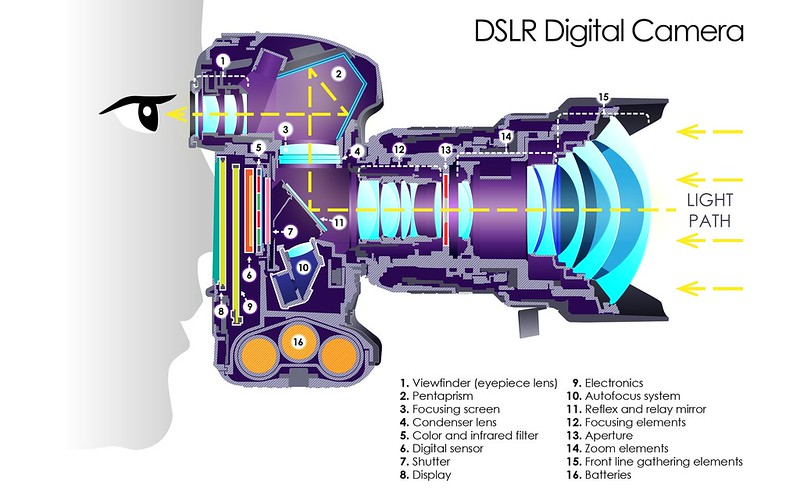
\includegraphics[width=\textwidth]{figures/light.jpg}}{Light}
    \caption{Camera and its various components \cite{cameracrosscut}.}
    \label{fig:camera}
\end{figure}

As was described in chapter \ref{ch:hvs}, digital cameras, to some extent, try to mimic the behaviour of the human eye. This attempt to mimic the human eye is achieved by combining optical elements like lenses, prisms and mirrors, mechanical elements like the shutter, and digital circuits like the imaging sensor. 

A crosscut of a typical digital single-lens reflex (DSLR) is shown in Figure \ref{fig:camera}. The camera can be seen as a light processor; each component takes in light, does some processing and passes it further for the next component to process. In the end, the photons reach the image sensor (6), where photoconversion occurs and are turned into digital units by the circuitry.

\section{Optical Systems}
\label{ss:optics}

Figure \ref{fig:optics} describes a basic ray diagram of image formation. An image of the object at a distance $d_0$ is projected to the image plane at a distance $d_i$, where the image recording material is placed. As the two rays coming from an object cross at the location of the image sensor, the resulting image is said to be in focus. The figure also shows the focal points $F$ and $F'$, which denote the location where parallel rays cross the optical axis. For an object at infinity, this is also where the object would appear in focus if we were to move the image plane from $d_i$ to $F$  \cite[159-183]{Hecht}.

Modern digital cameras, such as the one in Figure \ref{fig:camera}, consist of different lens elements of different shapes. The front elements (15) form the entrance pupil to capture as much light as possible from its surroundings and pass it to adjustable zoom elements (14), which enable the photographer to change the focal length to magnify onto subjects at various distances. The zoom elements are followed by the aperture (13) that allows us to control the amount of light reaching the sensor while keeping the rest of the elements in place \cite[159-239]{Hecht}.



\begin{figure}
\centering
\begin{tikzpicture}
    % Optical Axis
    \draw[->] (-4,0) -- (8,0) node[right] {Optical Axis};
    
    % Object
    \draw[thick] (-2,0) -- (-2,2) node[midway,left] {Object};
    
    % Lens
    \draw[thick] (0,-3) -- (0,3);
    \draw[->] (0,-3.2) -- (0,3.2) node[midway, xshift=0.5cm, yshift=0.5cm] {Lens};    
    % Focal Points
    \fill[red] (3,0) circle (2pt) node[below] {$F$};
    \fill[red] (-3,0) circle (2pt) node[below] {$F'$};
    
    % Image
    \draw[thick,blue] (4,0) -- (4,-1.5) node[midway,right] {Image};
    
    % Distance indicators
    \draw[<->, black] (-2, 2.5) -- (0, 2.5) node[midway, above] {$d_o$};
    \draw[<->, black] (0, 2.5  ) -- (4, 2.5) node[midway, above] {$d_i$};
    
    % Rays
    % Ray parallel to optical axis
    \draw[->,red] (-2,2) -- (0,2);
    \draw[->,red] (0,2) -- (3,0);
    \draw[->,red] (3,0) -- (4,-1.5);
    
    % Ray through F
    \draw[->,green] (-2,2) -- (0,0);
    \draw[->,green] (0,0) -- (4,-1.5);
    
\end{tikzpicture}

\caption{Basic image formation example.}
\label{fig:optics}
\end{figure}

Errors due to optical systems, such as colourful contours or gradual changes in brightness and colour shifts, are often attributed to how light bends when it passes from one medium to another. This phenomenon is governed by Snell's Law, which is typically presented as:

\begin{equation}
\label{eq:snell_revised}
n_1 \sin(\theta_1) = n_2 \sin(\theta_2),
\end{equation}

where $n_1$ and $n_2$ are the refractive indices of the first and second media, respectively, and $\theta_1$ and $\theta_2$ are the angles of incidence and refraction relative to the normal to the interface between the two media. However, dispersion is often omitted when discussing Snell's law, which specifies that the refractive index $n$ depends on the light's wavelength $\lambda$  \cite[108-109]{Hecht}. The refractive index can be more accurately represented as $n(\lambda)$, indicating its dependence on the wavelength. Therefore, a more precise formulation of Snell's Law that accounts for dispersion would include the wavelength dependence of the refractive indices:

\begin{equation}
\label{eq:snell_wavelength}
n_1(\lambda) \sin(\theta_1) = n_2(\lambda) \sin(\theta_2).
\end{equation}

This wavelength-dependent refractive index explains why light's different colours (wavelengths) bend at slightly different angles when passing through optical elements, leading to the optical errors observed in images. Three such errors are visualized in Figure  \ref{fig:aberration}, where light rays from a ring are first incident on a convex lens and finally reflected onto the image plane. In the topmost example, the ring is reproduced as seen in nature with no optical aberrations, as all light rays converge to the same location. In the second case, we see a noticeable blur along the edges of the ring; here, different light rays bend at slightly different angles due to dispersion, and as a result, each light ray has a different focal length, a phenomenon known as longitudinal chromatic aberration. In the third case, the light rays again converge at different locations due to dispersion, but at the same focal plane, thus this is called lateral chromatic aberration \cite[266-284]{Hecht}.

Shading is another issue arising from optics. It refers to the change in relative illumination from the centre of the captured image towards the edges, either as a decrease in luminance and/or variation in chrominance. They are respectively referred to as luminance and colour shading. Both can be characterized by taking an image under a uniform light source, known as a flat-field photograph. Uniform light can be achieved by using integrating spheres, which are typically highly uniform ($\ge$95\%) or placing a diffuser plate on top of the camera lens, spreading the incident light more evenly  \cite{ImageShading}.


Luminance shading, often referred to as vignetting, primarily results from a combination of the $cos^4(\theta)$ law, which states that there is a loss of illumination depending on the angle $\theta$, and shading related to mechanical and optical elements that might prevent some light rays from entering the sensor at particular angles. On the other hand, colour shading results from the combination of light hitting the wrong pixels due to steep angles of incidence (known as pixel cross-talk) and infrared (IR) filters, which have decreased performance when the angle of incidence increases. As such, these effects are primarily seen at the edges of the image  \cite[183-186]{Hecht}, \cite[251]{nakamura}, \cite{ImageShading}.


\begin{figure}
    \centering
    \pdftooltip{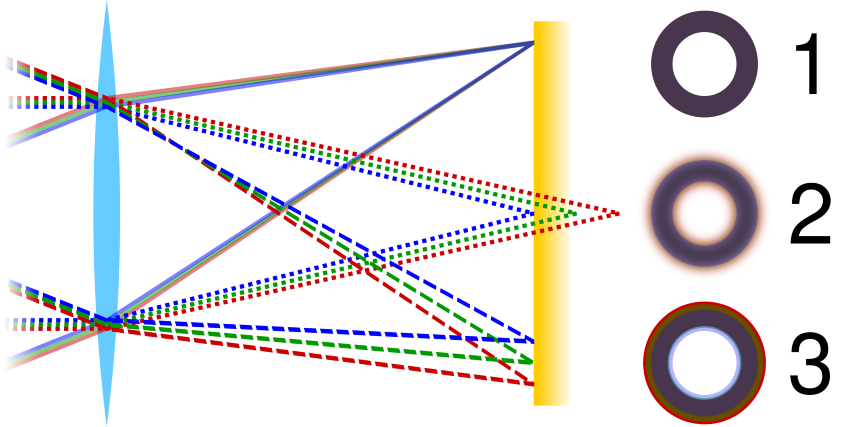
\includegraphics[scale=0.5, width=\textwidth]{figures/aberration.png}}{aberration}
    \caption{Optical aberrations \cite{aberration}. Ideal image (1), longitudinal chromatic aberration (2) and lateral chromatic aberration (3).}
    \label{fig:aberration}
\end{figure}

 
\section{Image sensors}

In the analogue era, photographic film was used to produce images, but it was slow due to the development process that had to be applied post-photography. Nowadays, the photosensitive material used is a semiconductor-based digital sensor, which converts incoming photons to electrons, resulting in an electric charge  \cite[272-274]{nakamura}. A crucial measure is then the photon energy, which is given by

\begin{equation}
\label{eq:photon}
{E_{photon}} = \frac{hc}{\lambda},
\end{equation}

where $h$ is the Planck's constant ($\approx \SI{6.626e-34}{J\cdot s}$), c is the speed of light
($\approx \SI{3e+8}{\meter\per\second}$) and $\lambda$ is the wavelength of the light. Since we have $\lambda$ in the denominator, the energy of a photon thus decreases with increasing wavelengths \cite[61-62]{Hecht} \cite[55-56]{nakamura}.

\subsection{Photoconversion}
\label{ss:photoconversion}
For a photon to convert into an electron, it must exceed the image sensor's band gap energy $E_{bg}$. However, as photons of increasing wavelengths penetrate deeper into the silicon, they begin to absorb at a lower probability. So, a photon with energy exceeding the band gap energy does not always result in an electron. A typical characteristic of an image sensor's ability to convert incident photons into electrons is its quantum efficiency (QE) \cite[77]{nakamura}. It tells us the proportion of photons that are, on average, converted into electrons and is given by the following equation: 

\begin{equation}
\label{eq:qe}
\text{QE}(\lambda) = \frac{\text{Number of electrons generated}}{\text{Number of incident photons}}
\end{equation}

The number of photons reaching a photosite depends on the exposure duration, so it is possible to compensate for quantum efficiency with more prolonged exposure durations, but generally, the better the quantum efficiency, the better the imaging sensor.

While quantum efficiency tells us how efficient the sensor is in converting photons into electrons, it does not consider the energy required to produce an electron with elementary charge $q$. From the formula in \ref{eq:photon}, it can be seen that photons with longer wavelengths have less energy, and as a consequence, it takes less energy to convert a long wavelength than a short wavelength photon into an electron. Knowing the quantum efficiency, it is then possible to compute the efficiency of photon conversion as a function of wavelength, known as the spectral responsivity (SR): 

\begin{equation}
\label{eq:sr}
\text{SR}(\lambda) =\text{QE}(\lambda) \cdot \frac{q}{E_{photon}} = \text{QE}(\lambda) \cdot \frac{q\lambda}{hc},
\end{equation}

Where QE is the quantum efficiency from \ref{eq:qe}, $E_{photon}$ is the energy of a photon for a given wavelength from \ref{eq:photon} and $q$ is the elementary charge of an electron \cite[78-79]{nakamura}.

In Figure  \ref{fig:qe}, we plot the normalized quantum efficiencies and spectral responsivities for each channel of the KAF-8300 image sensor by On Semiconductor in dashed and solid lines, respectively, in line with the formulas \ref{eq:qe} and \ref{eq:sr}, we see how, for the longer wavelengths, the spectral responsivities tend to increase relative to the corresponding quantum efficiencies. It thus takes less energy to produce a signal in the red channel than, for example, in the green channel of an image sensor.

\begin{figure}
    \centering
    \pdftooltip{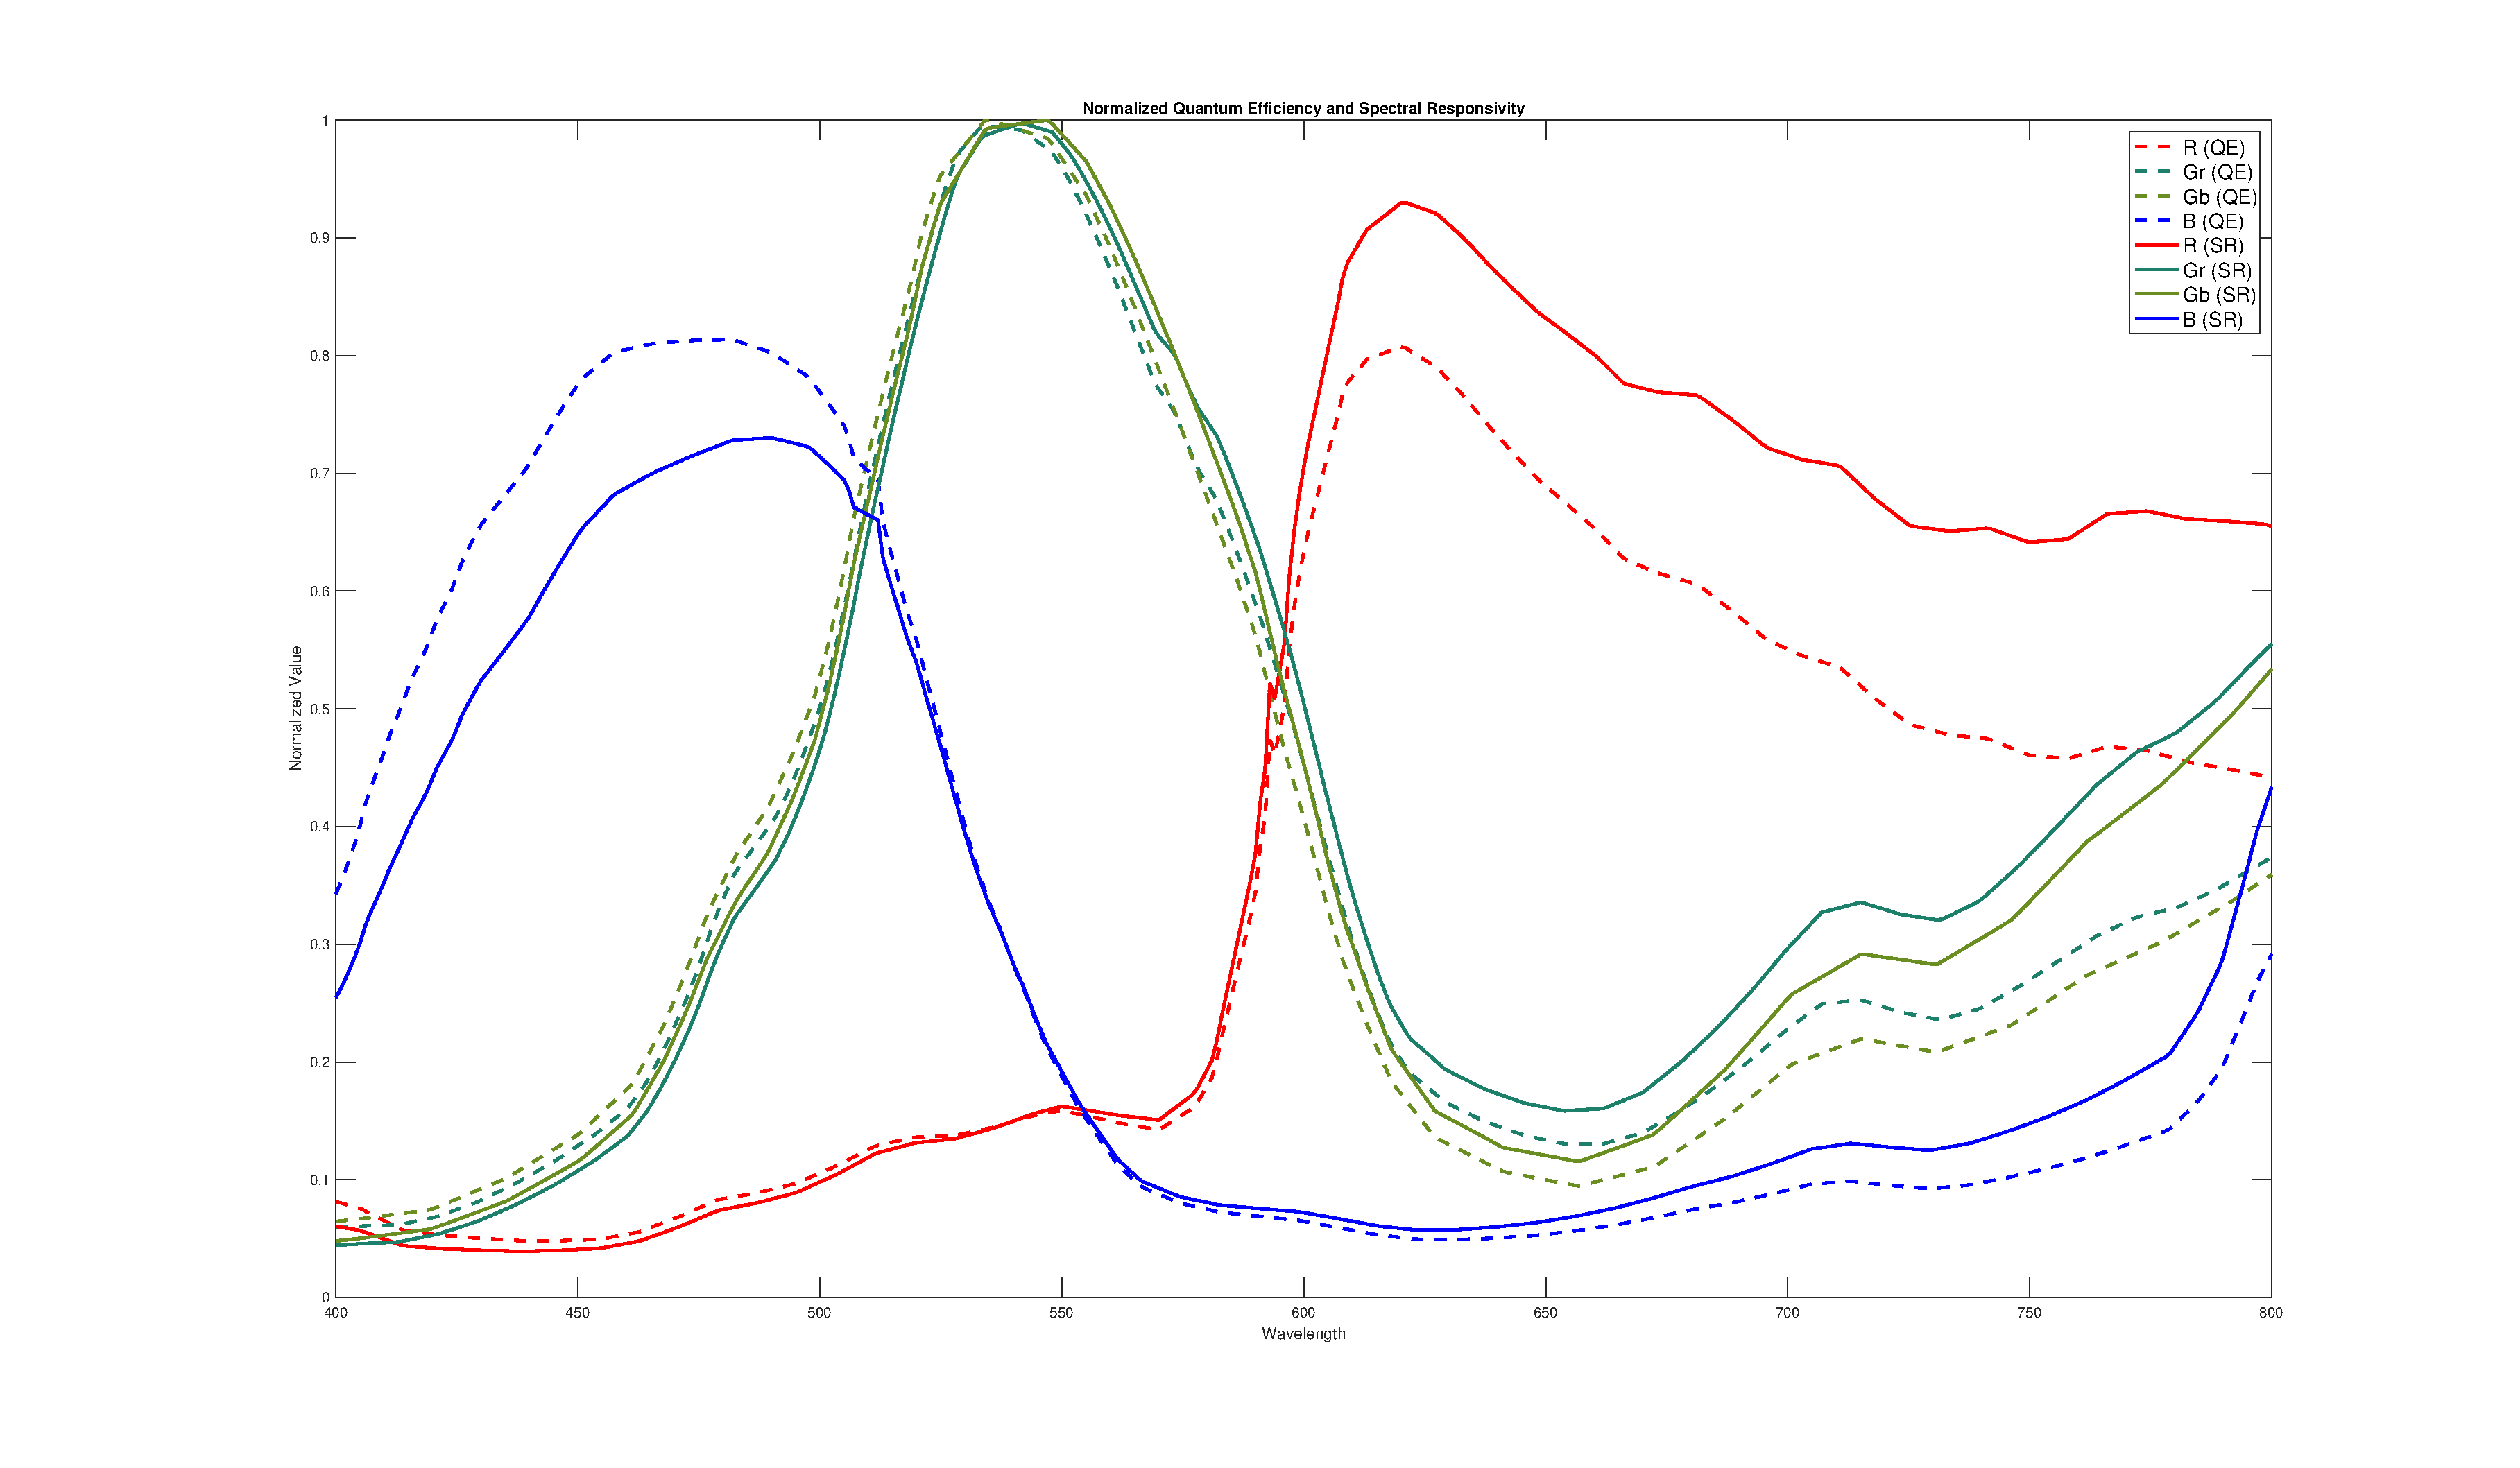
\includegraphics[width=\textwidth]{figures/normalizedqrsr.eps}}{SR}
    \caption{Normalized quantum efficiencies (dashed) and spectral sensitivities of KAF-8300 Image Sensor by OnSemi \cite{onsemi}.}
    \label{fig:qe}
\end{figure}

\subsection{Sensor types}

Currently, two dominant digital image sensor types exist:  Charge-coupled device (CCD) \\ and Complementary Metal–Oxide–Semiconductor (CMOS). Both operate similarly in \\ terms of photoconversion but differ in their internal process of converting the charge to a digital value. In both cases, colour information is achieved by placing optical filters on top of the imaging sensor, which will be discussed in \ref{ss:colour}  \cite[17]{nakamura}.

A diagram of the CCD structure can be seen in Figure \ref{fig:ccd}. The operation principle of a CCD sensor is based on having passive pixels that only collect charge and do no additional processing. When the shutter is opened, the pixels start to collect light until the shutter is closed again. Each pixel is overlaid with metal surrounded by insulating material that attracts electrons row-by-row into a serial shift register that propagates each electron into an amplifier, converting the small charge into a voltage. The movement of electrons is achieved due to their tendency to move towards a higher potential. So, by alternatively switching the voltage between adjacent pixels in a column, the electrons can be propagated downwards. The voltage is then converted to a digital value through an analog-to-digital converter (ADC)  \cite[95-139]{nakamura}, \cite[4]{Park2016}.


\begin{figure}
    \centering
    \pdftooltip{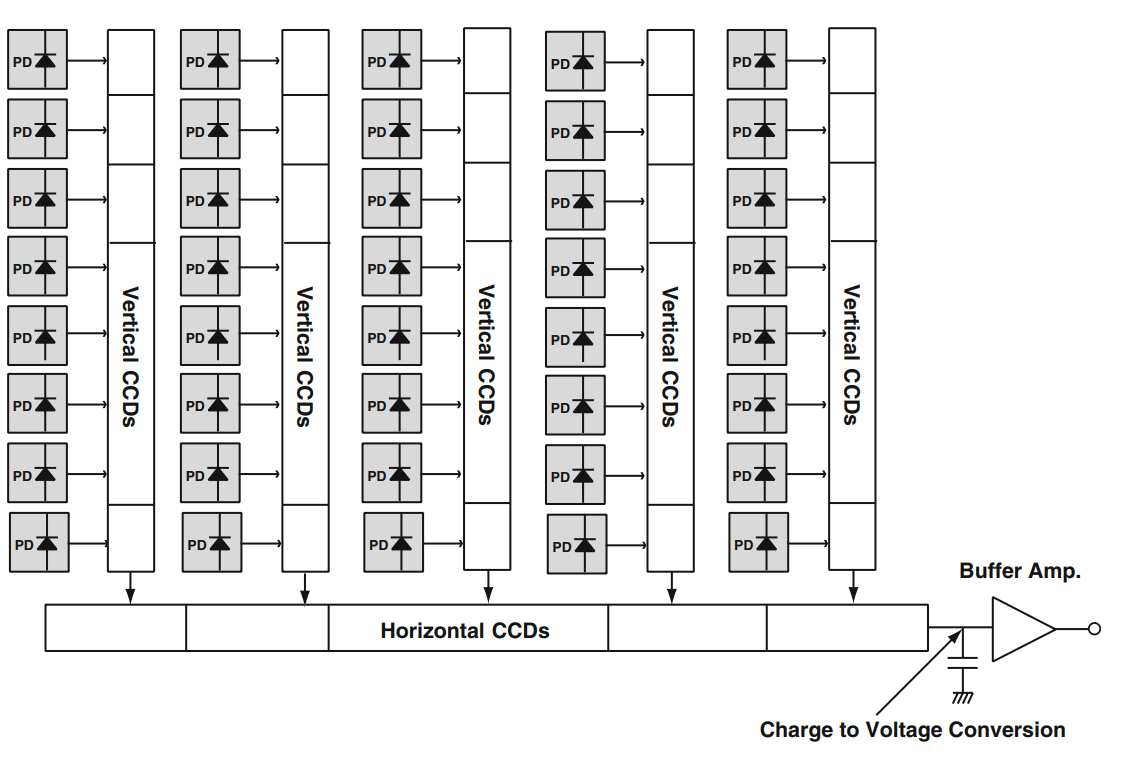
\includegraphics[width=\textwidth]{figures/ccd.png}}{CCD}
    \caption{CCD diagram. Figure copied with permission from the publisher \cite[4]{Park2016}.}
    \label{fig:ccd}
\end{figure}

 The CMOS sensor, for which the structure can be seen in Figure \ref{fig:cmos}, is more commonly used nowadays and takes an active pixel approach. An active pixel converts the charge to an analogue voltage at the photosite instead of sequentially processing each pixel through the same unit. The charges are then propagated row by row into an ADC. Since each pixel amplifies and converts to a voltage, the system can utilize parallelization efficiently. New designs might also have multiple ADCs, for example, per column, so the entire row can be converted into a digital value at once or at each photosite next to the amplifier, increasing the speed even further  \cite[144-176]{nakamura}, \cite[5]{Park2016}.

\begin{figure}
    \centering
    \pdftooltip{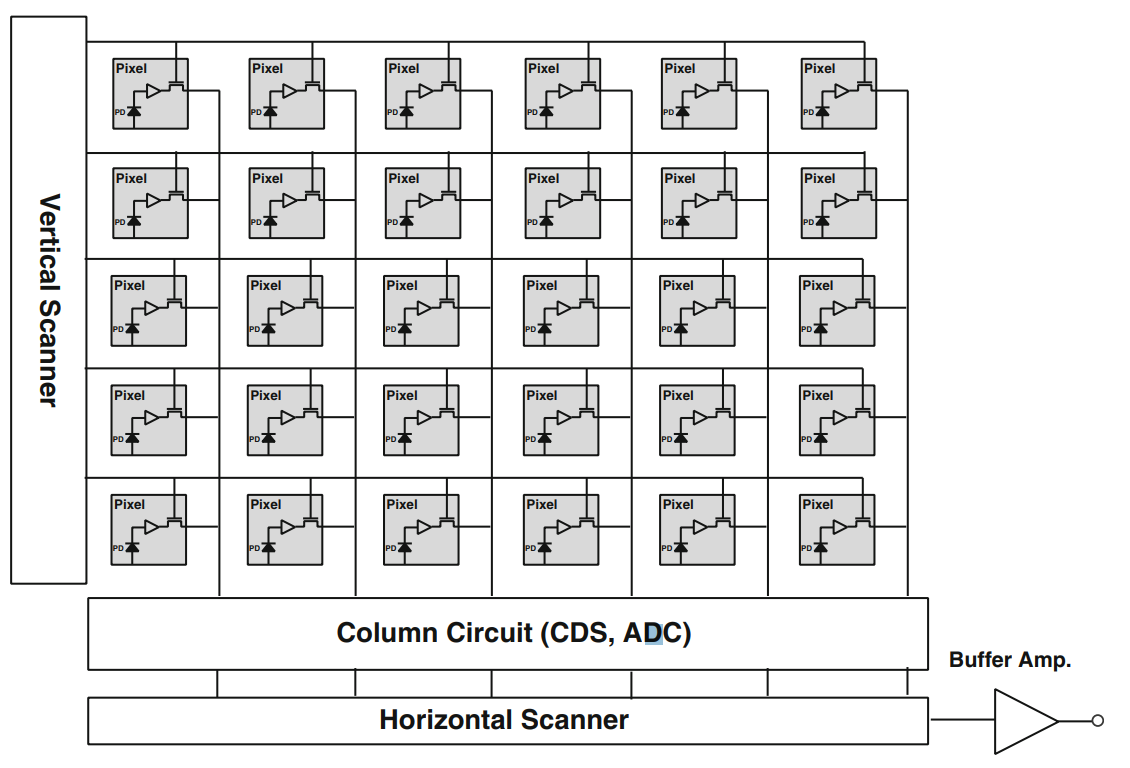
\includegraphics[width=\textwidth]{figures/cmos.png}}{CMOS}
    \caption{CMOS diagram. Figure copied with permission from the publisher \cite[5]{Park2016}.}
    \label{fig:cmos}
\end{figure}



\subsection{Pixel size}
\label{sec:fwc}

Cameras have been fitted into every mobile phone manufactured in the past decade. Since mobile phones are multi-purpose devices, the image sensors must not take up much space but still produce sharp, high-resolution images. The trick to downsizing image sensors from large digital single-lens reflex cameras (DSLRs) form factor has been to reduce the individual pixel sizes   \cite{xiao2009mobile}, \cite[308-309]{nakamura}.

The tradeoff with small pixels is that they cannot accumulate the amount of charge a large pixel would. Since a larger pixel also has a larger surface area, it can collect more photons during the exposure. A common analogy to this is to think of the different-sized pixels as buckets under a rainy sky, where each raindrop is a photon. As is shown in Figure \ref{fig:photonrain}, the result is that for different pixel sizes, the amount of collected water in proportion to the bucket size is the same for each bucket. However, as the giant bucket collects rain from a wider area, it collects more rain overall  \cite[2.27]{rowlands2020physics}. Analugous to the bucket volume, a pixel's amount of charge before saturating is known as \textbf{full-well capacity} (FWC) \cite[66]{nakamura}.

\begin{figure}
    \centering
    \pdftooltip{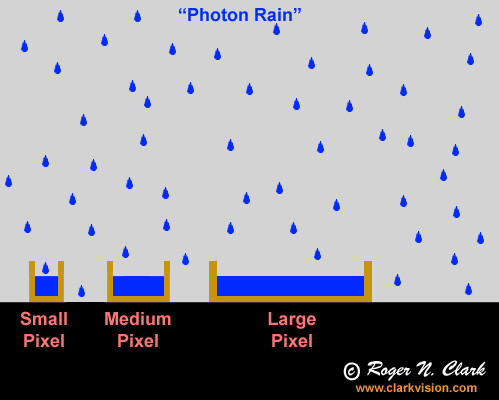
\includegraphics[scale=0.8]{figures/photon rain.png}}{PR}
    \caption{Photon rain \cite{clarkvision}.}
    \label{fig:photonrain}
\end{figure}

However, the number of photons emitted from a source per time period is not constant as expected but slightly varies. Because of their quantum nature, photons are discrete and independent of each other, making it impossible to observe fractional photon counts over any duration  \cite[61-67]{nakamura}. As such, the number of photons counted at a detector, such as an image sensor, follows a Poisson distribution:

\begin{equation}
\label{eq:poisson}
P(k; \lambda) = \frac{\lambda^k e^{-\lambda}}{k},
\end{equation}

where $\lambda$ is the mean of the distribution over a time period and $k$ is the number of realizations for a specific time period. For image sensors, the mean number of incident photons over multiple time periods (exposure times) can be taken as $\lambda$ and the number of photons for any individual period as $k$. 

For Poisson distribution, the variance is equal to the average, and so the standard deviation is the square of the mean, $\sigma = \sqrt{\lambda}$. Consequently, the SNR decreases as the average count of photons increases since the noise only grows as a square of the average signal level. This explains why noise is most prevalent when imaging in low-light conditions \cite[62, chapter. 3]{rowlands2020physics}.

\subsection{Colour Formation}
\label{ss:colour}

In the last section, we mentioned that spectral responsivity quantifies the energy required per wavelength to convert an electron into a photon. In this conversion process, the wavelength information is lost, as any photon exceeding the band gap level could have produced the electron. Image sensors are thus unable to distinguish colour and are monochromatic by nature.

The most common solution is an optical colour filter array (CFA), which forms a grid similar to the image sensor but filters light by its wavelength instead. Colour can be detected by designing the filters to allow light only in the red, green, or blue wavelength ranges. If we know the pattern of this filter, we have a rough idea of what kind of colour was incident on a specific pixel when reading the values recorded. A typical setup consists of identical blocks of 4 colour filters, a red, blue and two green filters. The reason for using twice as many green filters is that the human visual system is also more sensitive to the green wavelengths \cite[36]{Ramanath}, \cite[62-63]{nakamura}. This filter is also known as the Bayer filter after its inventor, Bruce Bayer \cite{Bayer1976}.

It is also possible to acquire colour information without a colour filter array. The most commonly known alternative, produced by Foveon, instead utilizes information about the silicon penetration depth to discriminate the colour of an incident photon \cite{lyon2002eyeing}, \cite{hubel2005foveon}. As was discussed in section \ref{ss:photoconversion}, higher wavelength photons penetrate deeper into the silicon, and thus, the colour of a photon can be read by measuring the charge generated at different depths. A diagram showing a high-level structure of a Foveon pixel is shown in Figure \ref{fig:foveon}. The main advantage of a Foveon sensor is that colour information is achieved at each pixel without demosaicking, unlike with Bayer colour filter arrays.

\begin{figure}
\centering
\begin{tikzpicture}

% Loop to draw the squares
\foreach \i in {0,1,2,3} {
    \foreach \j in {0,1,2,3} {
        \pgfmathtruncatemacro{\row}{mod(\i, 2)}
        \pgfmathtruncatemacro{\col}{mod(\j, 2)}
        
        % Choose color based on position
        \ifnum \row=0
            \ifnum \col=0
                \def\fillcolor{blue}
            \else
                \def\fillcolor{green}
            \fi
        \else
            \ifnum \col=0
                \def\fillcolor{green}
            \else
                \def\fillcolor{red}
            \fi
        \fi

        % Draw the square
        \fill[\fillcolor] (\i,\j) rectangle ++(1,1);
    }
}

\end{tikzpicture}
\caption{Color Filter Array.}
\label{fig:cfa}
\end{figure}

\begin{figure}
    \centering
    \pdftooltip{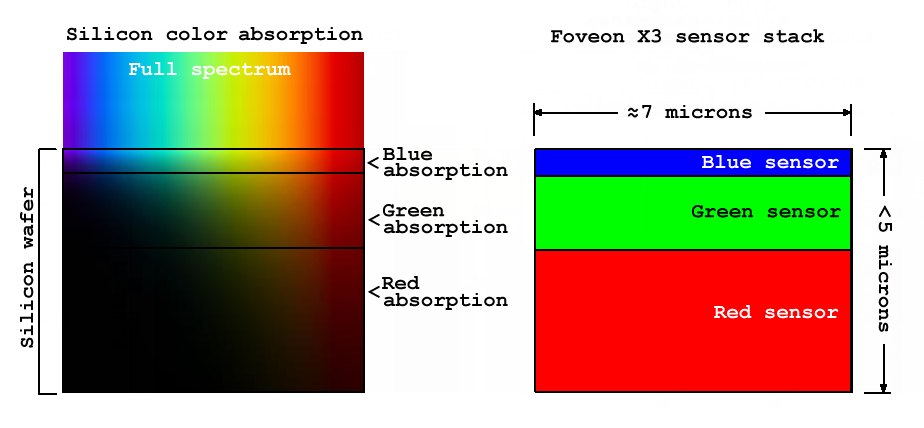
\includegraphics[width=\textwidth]{figures/foveon.png}}{Foveon}
    \caption{Colour sensing mechanism in Foveon sensors \cite{foveon}.}
    \label{fig:foveon}
\end{figure}


 The spectral sensitivities of the Nikon D5100 digital single-lens reflex camera (DSLR), measured by \citeauthor{D5100NPL}, are shown in Figure  \ref{fig:d5100}. It is apparent that since the green channel is relatively sensitive to all wavelengths, it would produce a higher response for an equal-energy (standardized as CIE E) illuminant than the other channels. Similarly, as for the human visual system, the imaging sensor computes its response to the incoming light by integrating the product of the illuminant's power spectral distribution, spectral reflectance of the object and the spectral responsivity of the sensor for a given colour over the wavelength range of interest.

\begin{figure}
    \centering
    \pdftooltip{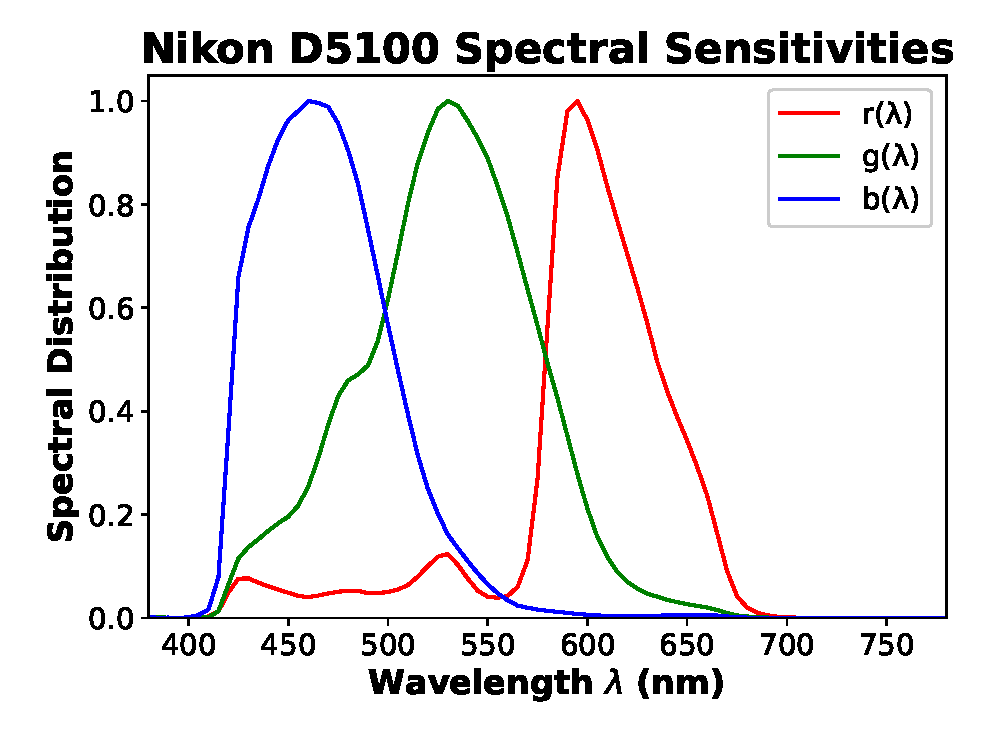
\includegraphics[width=\textwidth, scale=0.8]{figures/d5100_rgb.eps}}{nikon}
    \caption{Nikon D5100 Spectral Sensitivities  \cite{D5100NPL}.}
    \label{fig:d5100}
\end{figure}

\begin{subequations}
\begin{align}
\label{eq:sensor}
R = \int_{\lambda_{\text{min}}}^{\lambda_{\text{max}}} E(\lambda) R(\lambda) S_R(\lambda) \, d\lambda \\
G = \int_{\lambda_{\text{min}}}^{\lambda_{\text{max}}} E(\lambda) R(\lambda) S_G(\lambda) \, d\lambda \\
B = \int_{\lambda_{\text{min}}}^{\lambda_{\text{max}}} E(\lambda) R(\lambda) S_B(\lambda) \, d\lambda,
\end{align}

\end{subequations}

where $E(\lambda)$ is the spectral power distribution (SPD) of the illuminant, $R(\lambda)$ is the spectral reflectance of the imaged object and $S_T(\lambda)$ is the sensitivity of the sensor for tristimulus value $T$ (either $R$, $G$ or $B$). $\lambda_{\text{min}}$ and $\lambda_{\text{maxja }}$ are defined by the optical system, typically restricted to the visible range $\lambda_{\text{min}}$ = 380 nm and $\lambda_{\text{max}}$ = 780 nm.


\section{Image Signal Processing Pipeline}


Producing a perceptually pleasing image involves several processing steps typically executed within the camera. These steps are orchestrated by a computing unit known as the Image Signal Processor (ISP). The tasks within the ISP are divided into distinct blocks, which can operate in parallel or series, depending on the specific processing requirements \cite[91-101]{phillips2018camera}. Figure \ref{fig:dip} illustrates a typical colour image processing pipeline.

\begin{figure}
\centering
\usetikzlibrary{shapes.geometric, arrows}

\tikzstyle{startstop} = [rectangle,
minimum width=3cm, 
minimum height=1cm,
text centered, 
draw=black, 
fill=red!30]

\tikzstyle{io} = [trapezium, 
trapezium stretches=true, % A later addition
trapezium left angle=70, 
trapezium right angle=110, 
minimum width=3cm, 
minimum height=1cm, text centered, 
draw=black, fill=blue!30]

\tikzstyle{process} = [rectangle, 
minimum width=3cm, 
minimum height=1cm, 
text centered, 
text width=3cm, 
draw=black, 
fill=orange!30]

\tikzstyle{decision} = [diamond, 
minimum width=3cm, 
minimum height=1cm, 
text centered, 
draw=black, 
fill=green!30]
\tikzstyle{arrow} = [thick,->,>=stealth]

\begin{tikzpicture}[node distance=2cm]

\node (start) [startstop] {Raw Image};
\node (in1) [process, right of=start, xshift=2cm] {Black Level Subtraction};

\node (pro1) [process, right of=in1, xshift=2cm] {Lens Shading Correction};
\node (dec1) [process, right of=pro1, xshift=2cm] {White Balance};

\node (pro2a) [process, below of=dec1, yshift=-0.5cm] {Demosaic};

\node (pro2b) [process, left of=pro2a, xshift=-2cm] {Color Space Transform};
\node (pro2c) [process, left of=pro2b, xshift=-2cm] {Gamma};
\node (pro2d) [startstop, left of=pro2c, xshift=-2cm] {Post-Processing};



\draw [arrow] (start) -- (in1);
\draw [arrow] (in1) -- (pro1);
\draw [arrow] (pro1) -- (dec1);
\draw [arrow] (dec1) -- (pro2a);
\draw [arrow] (pro2a) -- (pro2b);
\draw [arrow] (pro2b) -- (pro2c);
\draw [arrow] (pro2c) -- (pro2d);

\end{tikzpicture}

\caption{Simplified colour image processing pipeline. Adapted from \cite{Ramanath}, \cite{JianpingZhou2007IPTf}.}
\label{fig:dip}
\end{figure}

Each block in the pipeline has adjustable parameters that can be fine-tuned to meet specific preferences or requirements. Image quality experts are often utilized in the industry to optimize these parameters and to perform experiments on subjective image quality, using, for example, ordinary people and their preferences \cite[29]{phillips2018camera}.


\subsection{Black Level Subtraction}

\begin{figure}
    \centering
    \pdftooltip{
\includegraphics[width=\textwidth]{figures/darkframe.jpg}}{darkframe}
    \caption{Dark frame taken on a Nikon D300, with enhanced contrast to highlight the noise \cite{darkframe}.}
    \label{fig:darkframe}
\end{figure}

Dark current is a noise source in photography, mostly prevalent at long exposures. It is also known as dark noise and can be observed by covering the camera lens entirely with a lens cap so that no light is incident on the sensor, and one would expect it not to record any voltage. However, this is wrong as the temperature around the sensor may cause electrons to be emitted, so a signal is recorded within the sensor. This type of noise can be characterized by measuring the average signal recorded under an environment where no light is incident on the sensor \cite[289]{nakamura}, \cite[63, chapter. 3]{rowlands2020physics}, \cite{Ramanath}. This image is often called a dark frame and is shown in Figure \ref{fig:darkframe}. To remove the effect of the dark noise on an image, the dark frame can then be removed from the following captured images. The process is often called Black Level Subtraction (BLS).

\subsection{Lens Shading Correction}

As was discussed in \ref{ss:optics}, lens shading results in the edges of the image having decreased brightness or variation in colour. The correction is typically performed by first characterizing the shading with a flat-field image, as was described in the same section. As this flat-field image has to be saved on the device for correction purposes, it is often downsampled before characterization into a look-up table of smaller size and interpolated at runtime \cite[251]{nakamura}, \cite{Park2016ISP}. This process is thus called Lens Shading Correction (LSC).

Luminance shading can be fixed by generating an inverse of the captured flat-field image, where the entries are the gain factors that must be applied to achieve similar brightness as in the centre of the image. \cite[286-287]{nakamura}. Depending on the optical system, the corners may sometimes be drastically darker in the flat-field image, and correcting them entirely in the digital domain would result in noisy corners. As such, the lens shading correction might not remove the shading altogether.

On the other hand, colour shading requires generating a similar correction table, but for each channel separately. Since for a uniformly illuminated image, it would be expected that the colour channels would be equal at every pixel location, the correction table is typically derived as a relative measure to some other channel's value \cite[286-287]{nakamura}. Since the green channel is typically the brightest in an image, the table is often generated by the ratio of red and blue values to the green values, $R/G$ and $B/G$.

\subsection{White Balance}
The concept of white balance (WB) in cameras, as explained in \cite[ch.~4.6]{rowlands2020physics}, is employed to replicate the phenomenon of chromatic adaptation discussed in section \ref{sec:chromaticadaptation}. WB is achieved by estimating the illuminant present in the scene and employing pre-defined multipliers to the pixel values that would equal the red, green and blue responses for an object that appears white to a human. As each illuminant might result in different proportions of red, green and blue responses for an object that appears white to a human, these multipliers are computed for a set of distinct illuminant types. This process, combined with colour correction (CC), cancels the effect of the illuminant and thus simulates the chromatic adaptation behaviour. 

The illuminant estimation algorithm primarily determines the accuracy of WB algorithms. A wrong estimation results in an improper choice of multipliers for colour correction (CC) and WB, leading to a distinct tint in the output image. Thus, the illuminant estimation process is perhaps the most important in the colour processing pipeline. For a review on illuminant estimation algorithms, we refer the reader to \cite{colourconstancy}.

Figure \ref{fig:wb} showcases the effect of applying WB. The images were simulated with Nikon D5100 spectral sensitivities \cite{D5100NPL} using scene reflectances from the dataset by \citeauthor{foster:2002} \cite{foster:2002}, under a D65 illuminant. Contrary to the figure in \ref{fig:dip}, demosaicking has been performed before white balancing. The left image has a noticeable green cast due to the spectral sensitivity imbalance between the channels. On the right side, it has been corrected by calculating the response to a Lambertian reflectance and the factors that make the channel responses even.

\begin{figure}
    \centering
    \pdftooltip{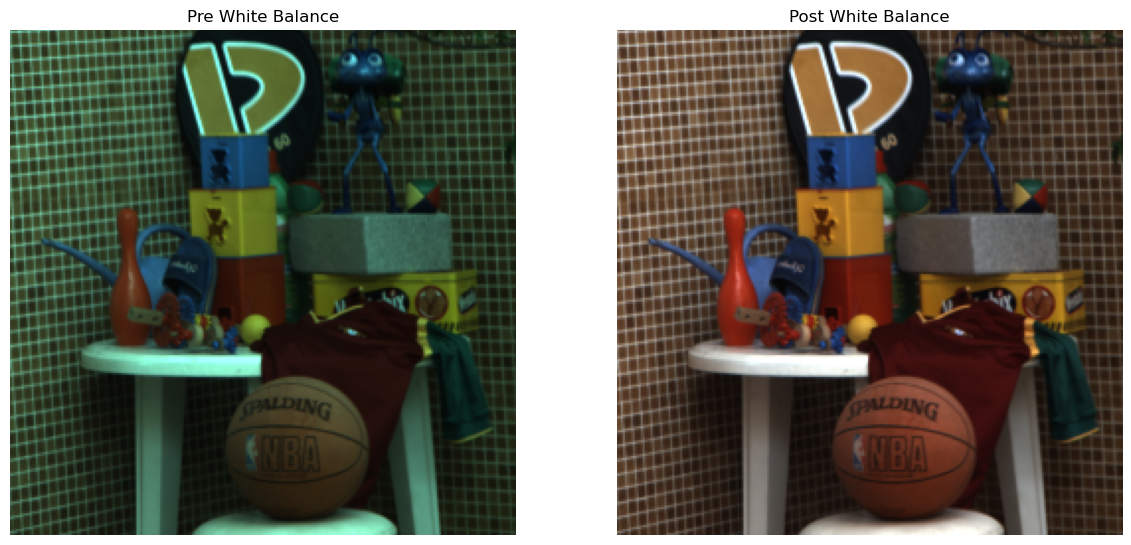
\includegraphics[width=\textwidth]{figures/wbnowb.png}}{wb}
    \caption{Scene before and after applying white balance, both with sRGB gamma applied. Image from Foster 2002 dataset \cite{foster:2002}. }
    \label{fig:wb}
\end{figure}

\subsection{Colour Filter Array Interpolation}

As discussed in Section \ref{ss:colour}, producing colour images begins with the image sensor being overlaid with a colour filter array. This array allows only light of specific wavelengths to pass through, a concept illustrated in \ref{fig:cfa}. The next step in creating a full-colour image involves a crucial process known as demosaicing.

Demosaicing employs various interpolation techniques to achieve colour accuracy. The simplest is the bilinear interpolation, based on direct interpolation methods. However, as documented in practical applications, these simple algorithms can sometimes fail, particularly at image edges \cite[46]{Ramanath}.

Acknowledging these limitations, researchers have developed more sophisticated algorithms. These advanced methods leverage cross-correlations between channels, adaptive filters, and frequency information. Such enhancements significantly improve the performance of demosaicing algorithms. Interested readers may refer to \cite{gunturk2005demosaicking} for a more detailed discussion.


\begin{figure}
    \centering
    \pdftooltip{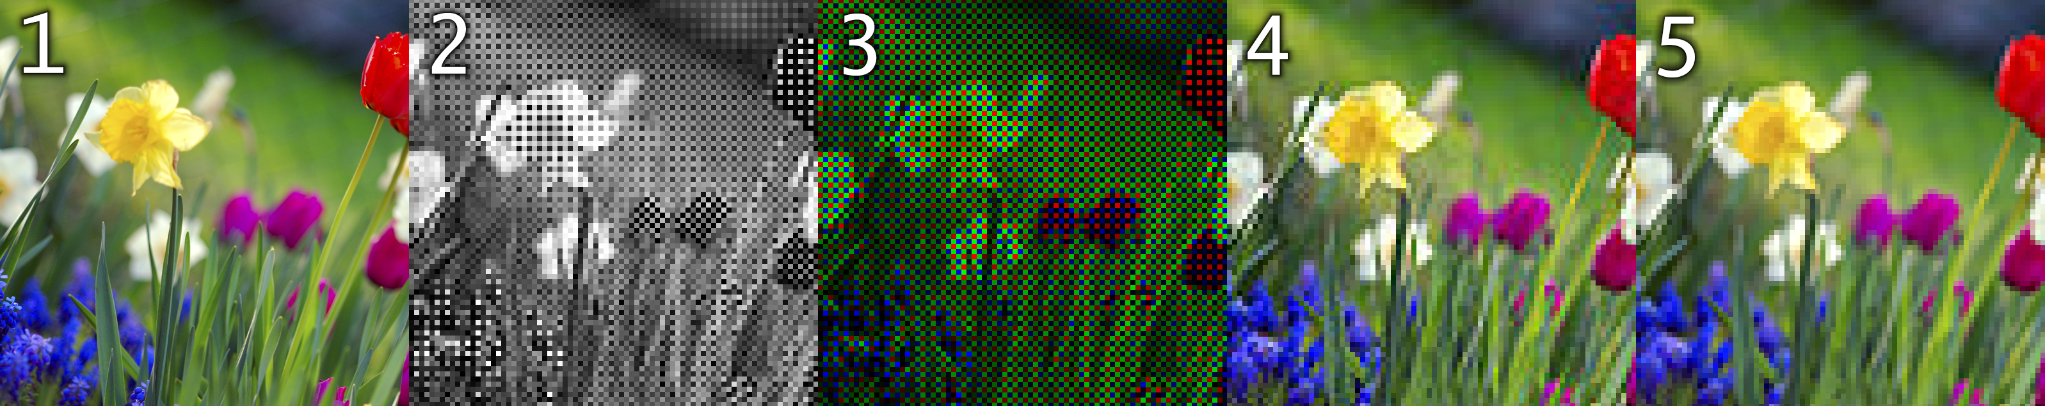
\includegraphics[width=\textwidth]{figures/horizontal_flowers.png}}{Demosaic process}
    \caption{Demosaic process \cite{demosaic}.}
    \label{fig:demosaic}
\end{figure}

\subsection{Colour Correction}
 \label{ss:cc}
Figures \ref{fig:xyz} and \ref{fig:d5100} demonstrate the significant differences in spectral sensitivities between the human eye and digital cameras, resulting in varying colour responses. Furthermore, the sensitivities can vary across different units of the same camera module \cite{walowit2019best}. In addition to colour inaccuracy, it also results in observer metamerism, where two cameras might see an object in differing colours while appearing the same for a human.

A colour correction matrix (CCM) is typically applied to the input image to account for the differences. The simplest way is to derive a 3x3 matrix by regression from camera responses to known XYZ responses for a standard observer. Like white balancing, this matrix is unique to each illuminant as white balancing only guarantees that neutral colours are mapped correctly \cite[1]{cheng2015beyond}. Furthermore, we can directly transform the input values to the desired output space, such as sRGB, with CCMs. This step is also often known as colour space transformation (CST).

Figure \ref{fig:cc} showcases the effect of colour correction, following a similar simulation process as in figure \ref{fig:wb}. On the left, we see the result of treating raw camera RGB values as sRGB values, resulting in an image with dull colours. On the right, colour correction has been performed to transfer the image from camera RGB to sRGB colour space, with the colours now being more saturated and vibrant.


\begin{figure}
    \centering
    \pdftooltip{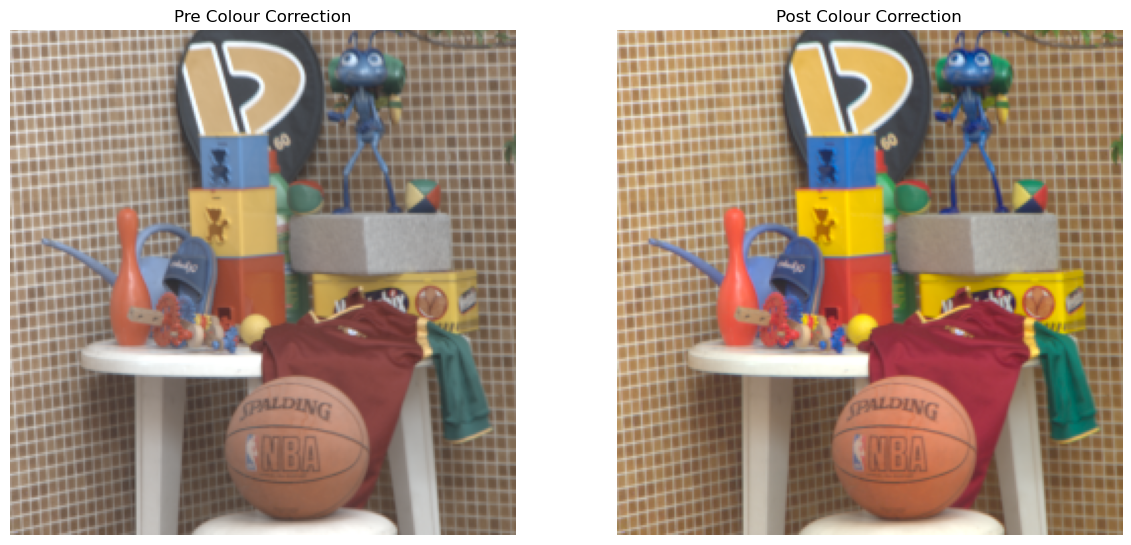
\includegraphics[width=\textwidth]{figures/cc.png}}{cc}
    \caption{Scene before and after applying Colour Correction, both with sRGB gamma applied. Image from Foster 2002 dataset \cite{foster:2002}. }
    \label{fig:cc}
\end{figure}


\subsection{Gamma}


Finally, the image has to be saved for storage. At this stage, the image is likely still in linear colour space, such as linear sRGB, and has to be transformed through a non-linear inverse gamma function to compensate for the monitor gamma \cite{4050037}. The gamma function is often modelled as follows:

\begin{equation}
V_{\text{out}} = V_{\text{in}}^\gamma,
\end{equation}

where $V_{\text{out}}$ is the output voltage after applying the gamma function, $V_{\text{in}}$ is the input voltage and $\gamma$ is the so-called decoding gamma. The camera pipeline thus applies the reciprocal gamma $V_{\text{in}}^{\frac{1}{\gamma}}$ at encoding phase. The effect of applying sRGB gamma to a set of greyscale values from black to white is displayed in Figure \ref{fig:gamma}. In the case of linear encoding, the gamma function is identity, so the output scales linearly with the scene's brightness. For sRGB encoding, the change from black to lighter greys is much more gradual and accurately represents how a human eye would perceive tones with a linear change in brightness.

\begin{figure}
    \centering
    \pdftooltip{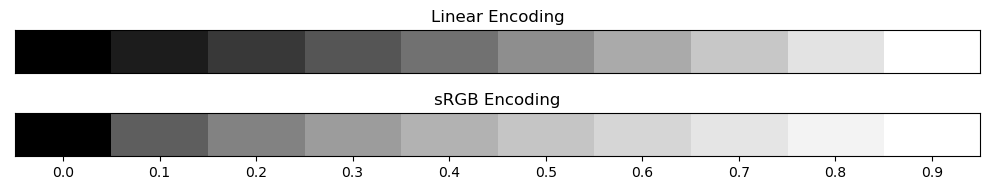
\includegraphics[width=\textwidth]{figures/gamma.png}}{gamma}
    \caption{Linear vs sRGB ($\approx 2.2$) Gamma Encoding.}
    \label{fig:gamma}
\end{figure}

Typically, the gamma is roughly $2.2$ to comply with colour spaces such as sRGB \cite{sRGB}. Inverse gamma was initially applied in images to compensate for non-linearities in CRT monitors. Still, it has also been found to closely simulate the human perception of brightness, which more accurately senses differences in darker tones. The input range becomes linear again when gamma decoding is performed on the monitor. When the image is viewed, the human eye performs its correction again, resulting in a similar perceived depth as stored.

\subsection{Post-processing}

In this phase, the process varies among manufacturers, focusing more on enhancing the image's visual appeal and ensuring it meets the intended output specifications. At this stage, the objective shifts from faithfully recreating the original scene to crafting an image representing an ideal version of what was observed.

Typical algorithms employed at this stage enhance the colours, for instance, by making them look more saturated and removing artefacts such as noise from the image. Sharpness is typically preferred, so an additional edge sharpening step is often performed  \cite[40-41]{Ramanath} \cite{4050037}.

Before display, the image is often compressed to save space. Some compression algorithms might discard information from the image that is not perceptually important to the viewer. Hence, they are often called lossy algorithms and convert the image into colour space with less correlation and detail across channels. Typical encoding formats encountered these days are some variants of JPEG \cite{JPEG} and PNG \cite{PNG}.



\chapter{Colour Correction}%
\label{ch:cc}

Colour correction is a step in the imaging pipeline responsible for producing images, that are understood by the display. As displays and cameras natively operate in different colour spaces, a mathematical transformation has to be performed. Moreover, each camera has slightly different spectral responsivities, which is why these transformations are unique for each manufactured camera. Due to this, the step is often called colour characterisation or colour space transformation.

\section{Problem formulation}

As was discussed before, the need for colour correction arises from the differences between the spectral responsivities of the human eye and the camera. A camera is said to be colourimetric if its spectral responsivities are a linear combination of the human eye responsivities, and so it satisfies the Luther-Ives condition \cite{luther, ives, nakamura}. This means that with just a linear transformation the digital camera could perceive colours as we humans do. Unfortunately, none do, and even if one did, it would be extremely difficult to manufacture at mass.

Camera manufacturers thus apply colour correction in the imaging pipeline as was seen in fig \ref{fig:dip}. Typically this is accompanied by the diagonal white balance matrix $D$, which replicates the chromatic adaptation behaviour for achromatic colours in the digital camera, ensuring whites and greys colours are mapped the same under every illuminant. However as the chromatic adaptation does not only apply to achromatic colours, it is then left for the colour correction matrix to compensate for the illuminant in chromatic colours. All colours are then corrected into an output-referred colour space with some reference white, such as sRGB with D65, and thus the effect of the illuminant of the scene is removed. A transformation matrix thus has to be defined for every illuminant, to the illuminant defined by the reference white of the output space.

The major reason for error in colour correction comes from incorrect estimation of the scene illumination, which results in incorrect white balance multipliers and CCMs for the correction process, which further amplifies the error. Furthermore, colour correction matrices are often derived for different light levels, sacrificing saturation for noise amplification \cite{satvsnoise}. If the estimation of the scene light level is incorrect, we may pick the wrong matrix and amplify the noise. To alleviate this, we can impose constraints on the optimization process, to enforce smoothness in the coefficients of the matrix and ensure the saturation is within certain limits.

\section{Mathematical formulation}
\chapter{Proposed Method}
\label{ch:proposal}

In this thesis, we present a new algorithm for colour correction. We take the polynomial regression model further by utilising piecewise polynomials, specifically splines. The piecewise property enables polynomials of varying smoothness to be fitted across the function domain. Although different types of splines exist, basis splines (B-splines) are often used due to their minimal support, which means they can be fitted locally. This allows us to restrict sharp changes in the function shape to a restricted domain, unlike with polynomials \cite[140]{HastieTrevor2009EoSL}.

The idea of using splines for colour correction came upon reading \cite{finlayson2015color}. An observation of the smoothness of the fit was particularly emphasised, which is why they initially proposed the root polynomial model. The idea was based on the fact that reflectance spectra are usually relatively smooth, and linear models already perform exceptionally well. Furthermore, the spectral sensitivities of an image sensor and cones are relatively close, so a good fit is achievable with little non-linearities. Similar observations, albeit for scanners, were also discussed in \cite{wandell1993water}.

\section{Splines}

Splines belong to the family of piecewise polynomials but have constraints that make them convenient for fitting smooth functions. The boundary of each interval is known as a \textbf{knot}. For regular piecewise polynomials, the function values at knots are not constrained, and thus we may run into discontinuities \cite[141-144]{HastieTrevor2009EoSL}. This effect is shown in the top left plot in Figure \ref{fig:discontinuity}, where age is plotted against wage. At $Age=50$, there is an apparent discontinuity in the fitted function, although it still captures the shape of the data well.

In the top right plot in Figure \ref{fig:discontinuity}, we see another attempt to fit a polynomial to the data, but this time with a constraint that the two functions must be joined at the knot, making it continuous. This, however, creates a corner at $Age=50$, and the analytical derivative is not defined at that point. Consequently, the function is not very smooth at this point.

\begin{figure}
    \centering
    \pdftooltip{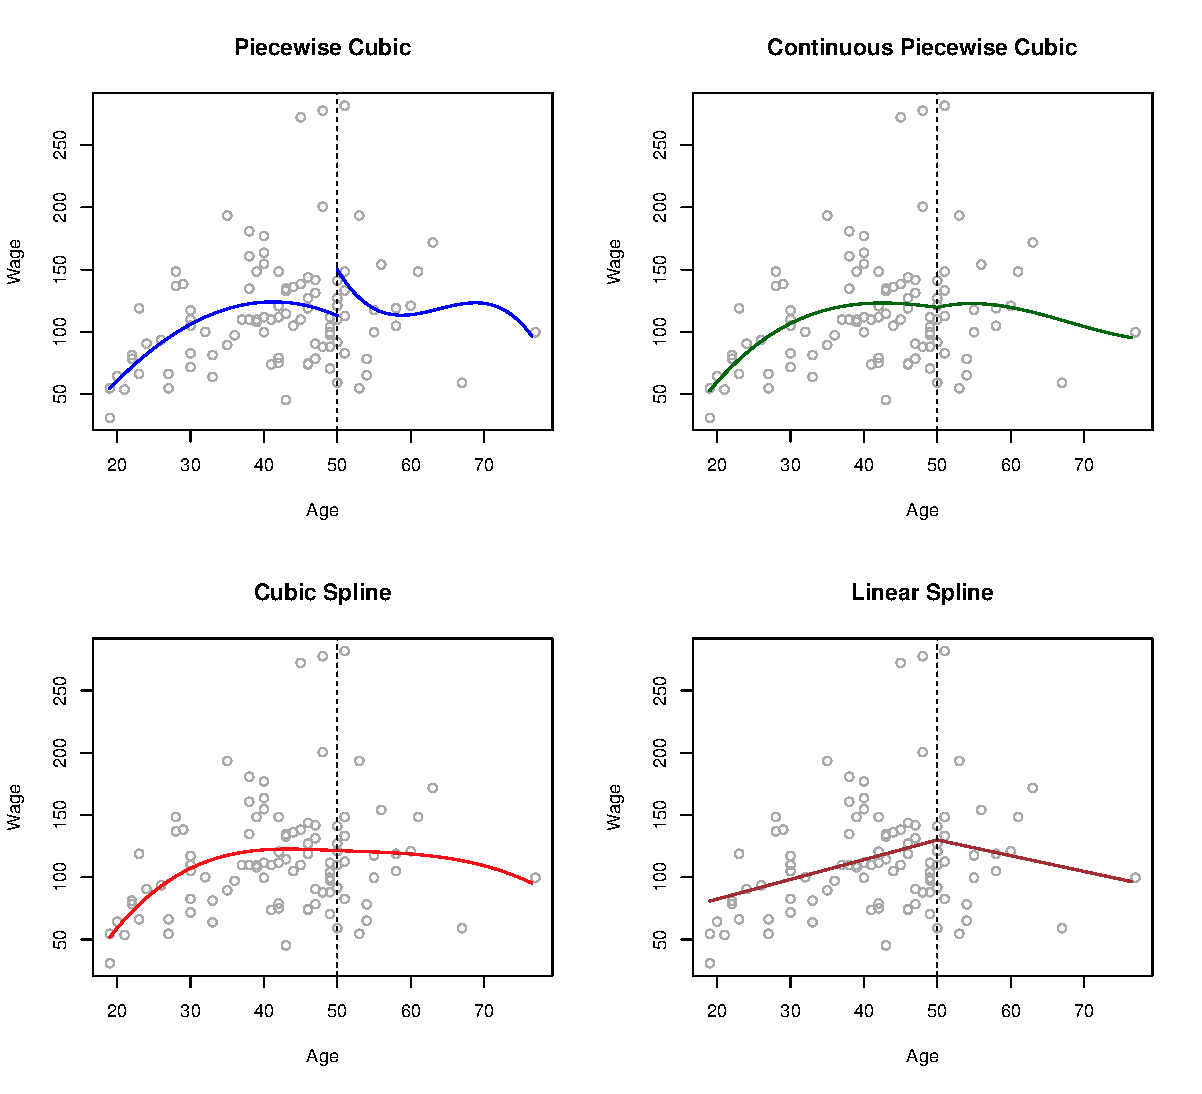
\includegraphics[width=\textwidth]{figures/7_3.pdf}}{piecewise polynomial}
    \caption{Piecewise polynomial fit with discontinuity \cite[295]{JamesGareth2023AItS}.}
    \label{fig:discontinuity}
\end{figure}

Finally, two spline model fits are shown at the bottom of Figure \ref{fig:discontinuity}. For a degree $d$ spline ($d=33$ for cubic, $d=1$ for linear), there is a constraint that the derivatives are continuous up to degree $d-1$ \cite[296]{JamesGareth2023AItS}, \cite[187]{HastieTrevor2009EoSL}. For the left plot, we thus have a guarantee that all derivatives up to degree 2 are continuous. In contrast, for the linear spline in the right figure, we only have a requirement that the function's first derivative is continuous, which is accurate as it is just a constant.

The order and the knots thus parametrise splines. For the former, there are two parameters we can tune: the position and number of the knots. The choice of location of the knots usually depends on whether we have some domain knowledge about the problem, e.g., knowing the locations of abrupt changes in the function. Otherwise, the knots can be placed at uniform distances or based on the data distribution (quantiles). The number of knots can be chosen similarly from the assumptions of the function shape  \cite[186-189]{HastieTrevor2009EoSL}.

\subsection{B-splines}

Perhaps the most important family of spline functions is formed by \textbf{basis splines}, commonly known as B-splines. The name comes from the fact that all other types of splines can be approximated by linear combinations of B-splines, acting as a basis for the family of splines.\cite[87-93]{practicalguidetosplines} An example of a different order B-splines was seen in the bottom row of \ref{fig:discontinuity}, where 3rd and 1st order functions were used respectively.

As stated before, all B-spline functions are defined as a linear combination of lower-order splines. Unlike polynomials, a spline of order $M$ consists of polynomials of degrees $M-1$ due to the continuity condition at the knots. Increasing order of B-splines can then be computed recursively given the first-order spline formula:

\begin{equation}
B_{i,1}(x) = 
\begin{cases} 
1 & \text{if } \tau_i \leq x < \tau_{i+1} \\
0 & \text{otherwise}
\end{cases}
\end{equation}

\text{for } i = 1, \ldots, K + 2M - 1, where $K$ is the number of knots and $\tau_i$ and $\tau_{i+1}$ denote the \textbf{support} of the function. Generally, a spline of order $M$ also spans $M$ knots, and thus, for a 1st order spline, we have that the constant function spans a single knot \cite[186-189]{HastieTrevor2009EoSL}.

A B-spline of order $M$ is the sum of two shifted order $M-1$ B-splines at the current knot position $i$ and the next knot position $i+1$. The formula is then given by: 
\begin{equation}
\label{formula:splines}
B_{i,m}(x) = \frac{x - \tau_i}{\tau_{i+m-1} - \tau_i} B_{i,m-1}(x) + \frac{\tau_{i+m} - x}{\tau_{i+m} - \tau_{i+1}} B_{i+1,m-1}(x)
\end{equation}
\text{for } i = 1, \ldots, K + 2M - m. \cite[186-189]{HastieTrevor2009EoSL}, \cite[90]{practicalguidetosplines}.

Figure \ref{fig:spline} displays the first three B-spline functions of non-zero order. As in equation \ref{formula:splines}, the splines recursively utilise adjacent lower-order splines in the formation, it can be observed that the higher-degree splines are also non-zero for a wider area. This is also apparent from the property that a nth order spline spans $M+1$ knots and is also evident from formula \ref{formula:splines}, where the subsequent interval is also always considered.

\begin{figure}
    \centering
    \pdftooltip{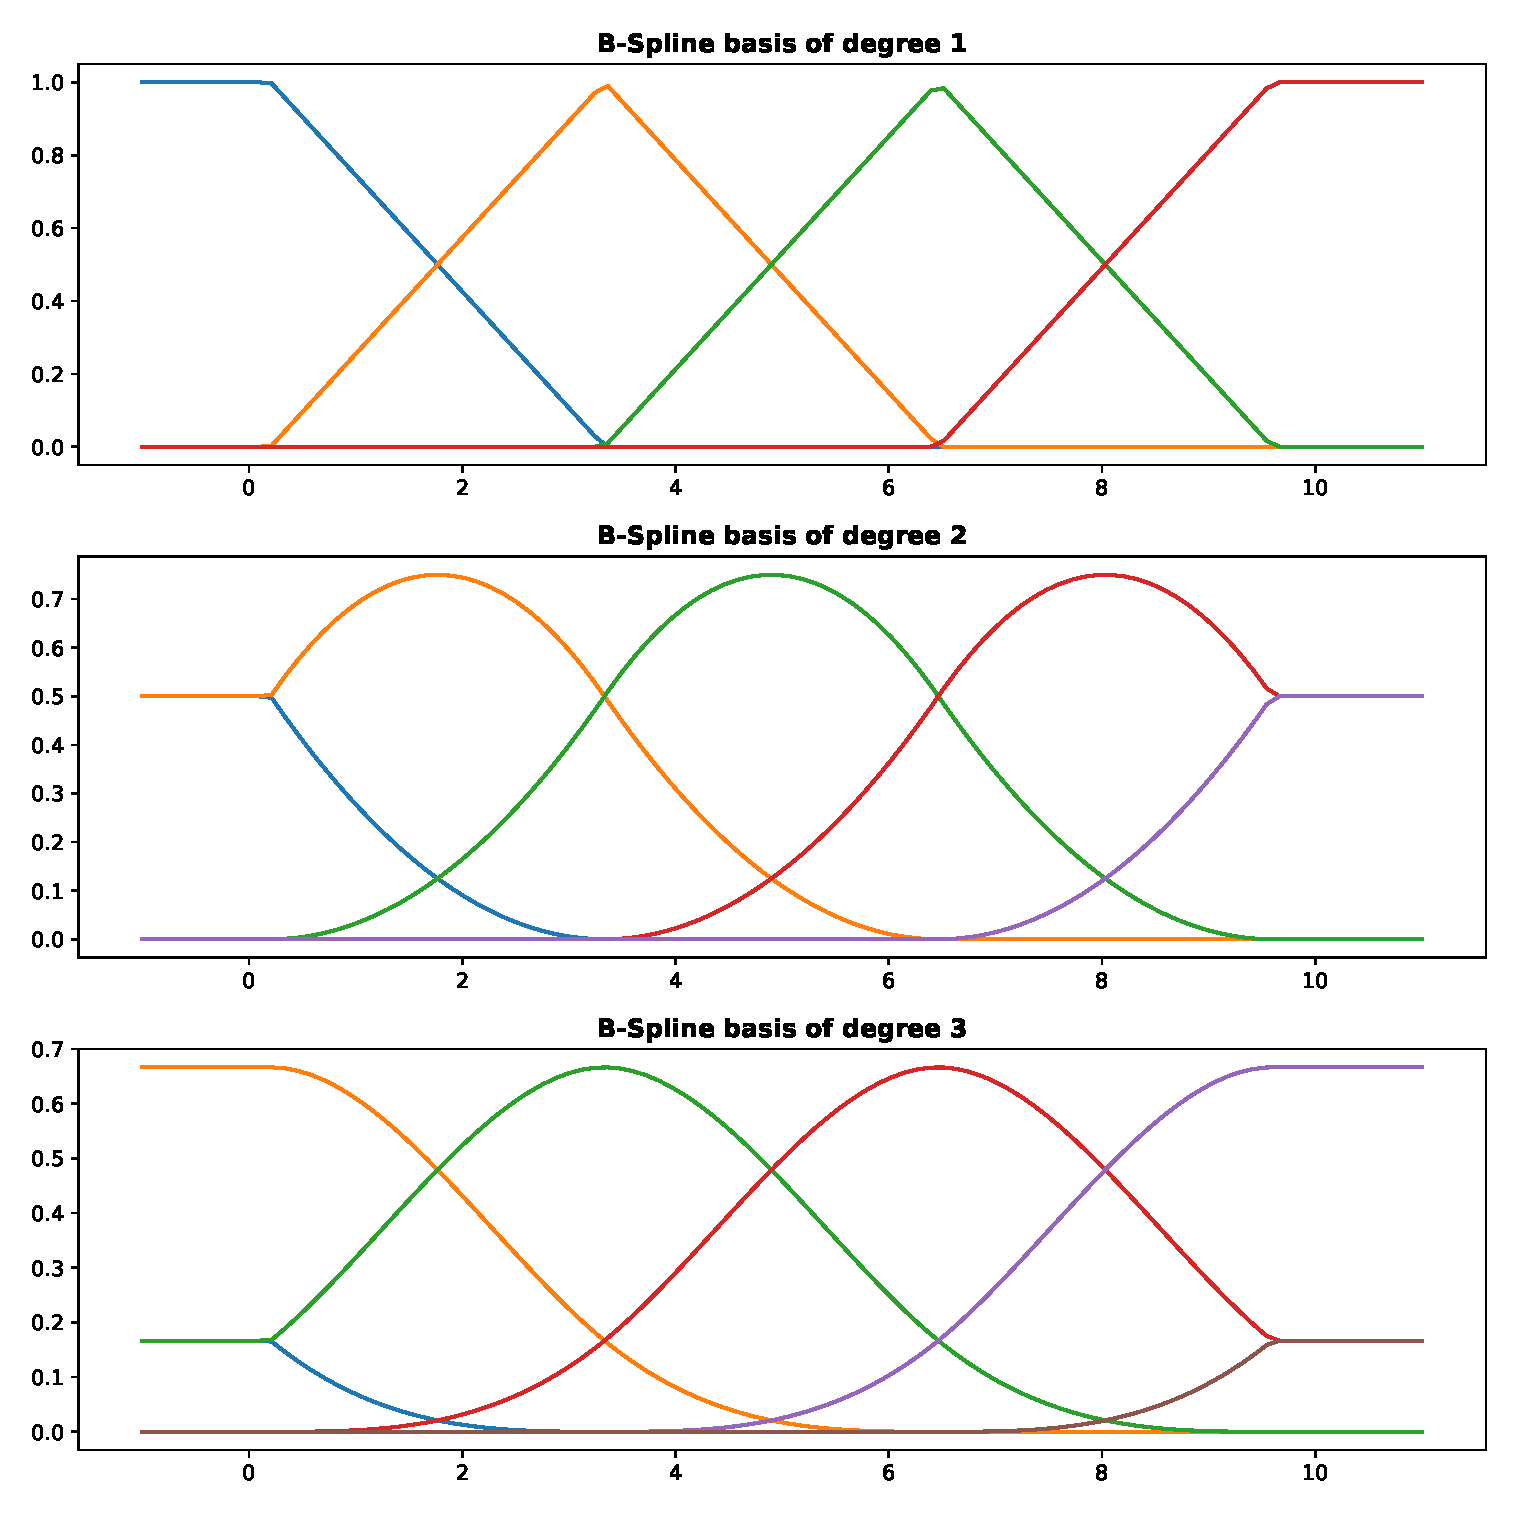
\includegraphics[width=\textwidth]{figures/splines.eps}}{B-Spline basis functions}
    \caption{Spline basis functions visualised}
    \label{fig:spline}
\end{figure}

Theoretically, this should allow us to approximate a large family of functions with linear combinations of B-splines. For example, in regression problems, we can utilise basis transformations of the original variables as new features. The output is then a linear combination of the B-spline features and may well approximate another spline function without us explicitly finding the correct basis.

\subsection{Tensor Product Splines}

As was seen in \ref{ss:polynomials}, polynomial models often utilise interactions between the original features as new features. This is carried out by a simple multiplication of the features. Up to two variables, these can be visualised as surface approximating the target output, which offers intuition on the nature of the fit.

Utilising interactions between variables, as was done with polynomial models, is also straightforward with splines via tensor products. Assuming we have transformed our red and green channel features using $n$ splines per feature, the interactions would be captured as follows:

\begin{equation}
\label{tensorspline}
\mathbf{r} \otimes \mathbf{g} = \mathbf{r} \mathbf{g}^T =
\begin{pmatrix}
r_1 g_1 & r_1 g_2 & r_1 g_3 \\
r_2 g_1 & r_2 g_2 & r_2 g_3 \\
r_3 g_1 & r_3 g_2 & r_3 g_3 \\
\end{pmatrix},
\end{equation}
where $\mathbf{r}$ and $\mathbf{g}$ are $n \times 1$ vectors containing the values of the $n$ B-spline basis evaluated at the position of the input pixel's intensity level for the red and green channels. All two-way interactions can then be considered using three tensor-product matrices: $\mathbf{r} \otimes \mathbf{g}$, $\mathbf{r} \otimes \mathbf{b}$ and $\mathbf{g} \otimes \mathbf{b}$. Combining these into one matrix forms our design (or basis) matrix for regression.

The beauty of this is that we can now assign each tensor product term its term and control the shape of the regression surface more effectively. An example of a surface generated by a tensor product spline of two variables can be seen in Figure \ref{fig:tensorspline}.

A downside to tensor product splines is the curse of dimensionality \cite[163]{HastieTrevor2009EoSL}. As we increase the number of features or splines per feature, the dimension of our feature matrix increases quadratically. In practical implementations, especially when running on low-power embedded devices, there is thus a trade-off between possible performance gains and computing resources. 

\begin{figure}
    \centering
    \pdftooltip{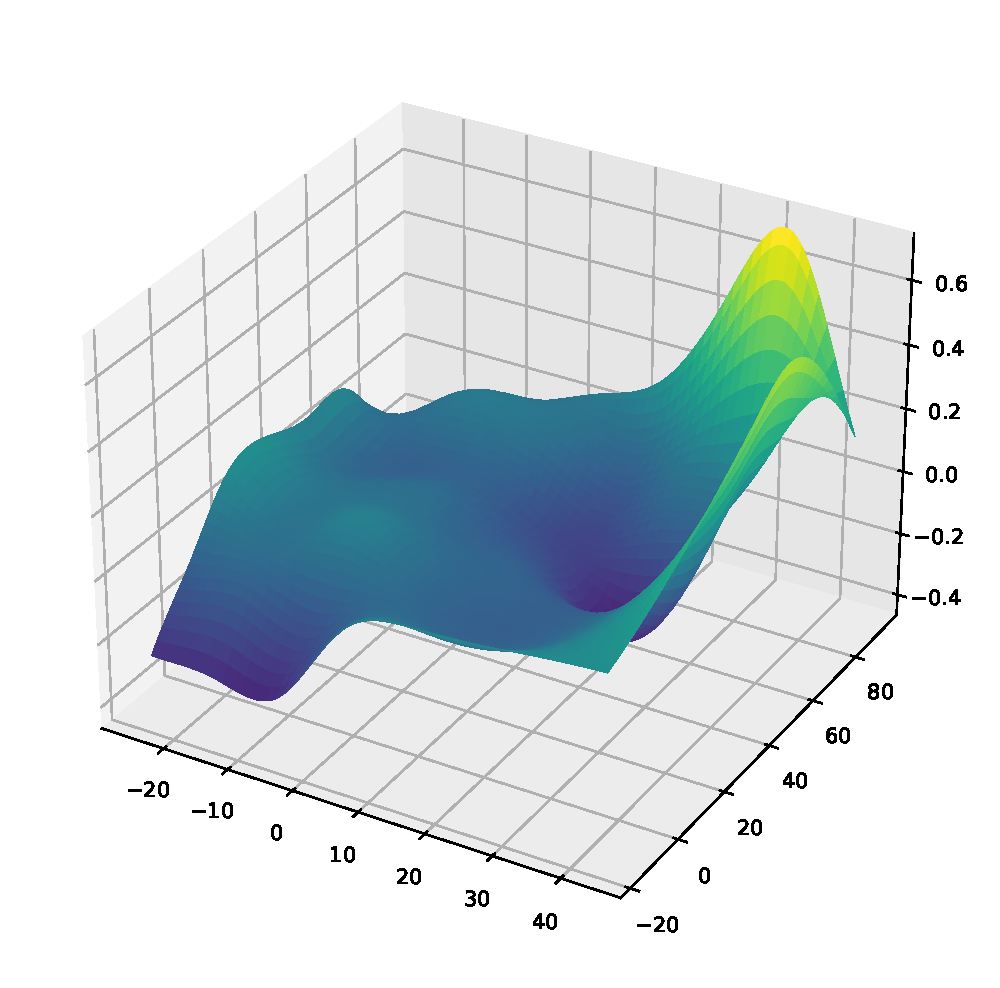
\includegraphics[scale=0.7]{figures/tensorspline.eps}}{Tensor Product Splines}
    \caption{Partial dependence visualisation of a tensor product spline term.}
    \label{fig:tensorspline}
\end{figure}

\section{Penalised B-splines for Colour Correction}

The primary research output of this thesis is the use of an extension of B-splines, known as Penalised B-splines. In the previous section, we saw how splines allow us to extend our basis into a new one with fine-grained control through piecewise polynomials. We also discussed how the dimension of the basis grows exponentially when we introduce interactions between splines. Here, we introduce the origins and theory behind our model.

\subsection{Model Regularization}

An issue commonly discussed in the Machine Learning (ML) communities is overfitting. This happens when the model is too complex and begins to fit precisely to the data points in our training set. Often, this is not desired, as the training data is just a subset of the samples we see in the real world, and the surface might fit poorly to unseen data. Often, the way to combat this is to increase data by collecting more real-world samples or augmenting the data, for example, by adding noise to the existing samples. This effect is visible in Figure \ref{fig:overfit}, where an overly complex polynomial model is fit to noisy sinusoidal data.

Another way to prevent overfitting is by introducing a penalty term to the least-squares problem. 
This is called regularisation, and often methods are used, such as Ridge \cite{hoerl2000ridge} and Lasso \cite{tibshirani1996regression} regression. They minimise the coefficients' L2 and L1 norms, resulting in a more numerically stable range of values for coefficients, especially for models where the features are correlated.\cite[61-69]{HastieTrevor2009EoSL} In these cases, we often observe large coefficients when using regular least-squares techniques.

\begin{figure}
    \centering
    \pdftooltip{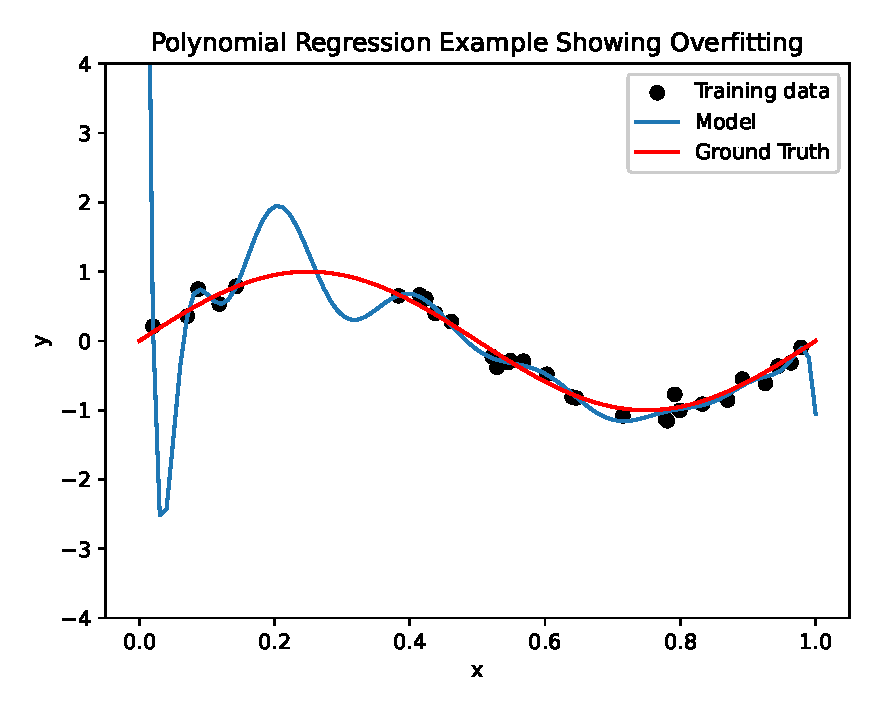
\includegraphics[scale=0.8]{figures/overfit.eps}}{Example of overfitting}
    \caption{Example of a high-degree polynomial model overfitting a noisy sinusoidal data}
    \label{fig:overfit}
\end{figure}

Another way to regularise a regression model with many predictors is to penalise the second derivative of our predictors. Second derivatives correspond to the curvature of our function, and as such, the penalisation term attempts to fit a line or a hyperplane to the data. Often these are paired with least-squares objective, which attemps to interpolate the training data. The balance between these two is determined by the smoothing parameter $\lambda$ in the following way:

\begin{equation}
\text{RSS}(f, \lambda) = \sum_{i=1}^{N} \left\{ y_i - f(x_i) \right\}^2 + \lambda \int \left\{ f''(t) \right\}^2 dt,
\label{formula:smoothingsplines}
\end{equation}

where $y_i$ are the target samples, $f(x_i)$ are the interpolating functions, and $\lambda$ controls the effect of the penalty term on the loss. These are often called Smoothing Splines, although $f(x_i)$ can also be any other function and is picked based on which minimises the loss. \cite[151]{HastieTrevor2009EoSL}

\subsection{Penalized B-Splines}

Penalised B-splines (P-Splines) were first proposed by \citeauthor{eilers1996flexible} in 1996 \cite{eilers1996flexible}. Their formulation is similar to that of smoothing splines in \ref{formula:smoothingsplines}, but they instead penalise the difference of coefficients in adjacent splines. They are then defined as follows:

\begin{equation}
\|\mathbf{y} - \mathbf{B}\boldsymbol{\alpha}\|^2 + \lambda \|\mathbf{D}\boldsymbol{\alpha}\|^2,
\label{formula:psplines}
\end{equation}

where $\lambda$ again controls the penalty term, $\mathbf{B}$ and ${\alpha}$ are the design matrix of basis functions and coefficients. $\mathbf{D}$ is known as the difference matrix, and multiplying $\alpha$ with it computes the nth order differences of $\alpha$. For example, the first-order difference between adjacent coefficients would be $(\alpha_j - \alpha_{j-1})^2$. \cite{eilers2021psplines}

With P-splines, it does not harm to have a too large basis if computational complexity is not a concern. Selecting the smoothing parameter appropriately is quickly done by a simple grid search. In Figure \ref{fig:largebasis} we see this property of P-splines in action, with the basis functions scaled by their coefficients in different colors. Despite the number of basis functions being much larger than the number of training samples, the produced curve is smooth and does not overfit the data. It is thus safe to pick excessively too many basis functions initially, visualise the produced surface and restrict their number if the computation becomes a bottleneck. \cite{eilers2021psplines} An initial model might act as a starting point for analysing the nature of the transformation at hand before any optimisations.


\begin{figure}
    \centering
    \pdftooltip{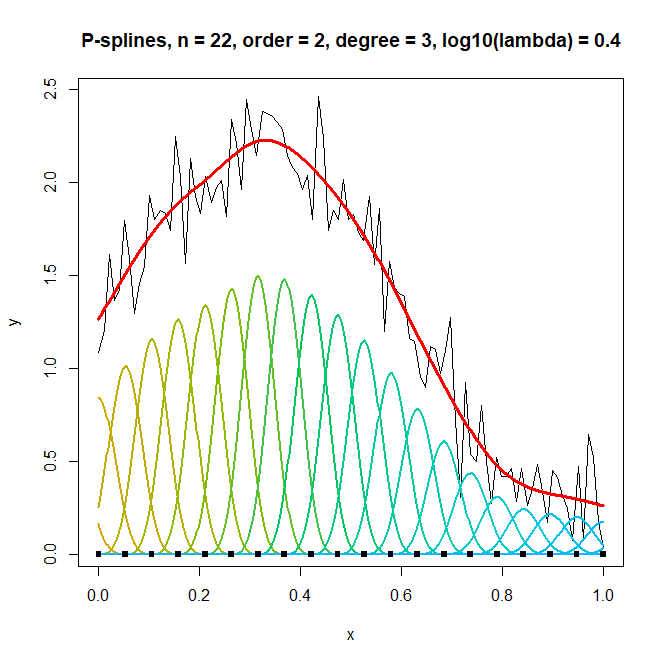
\includegraphics[scale=0.5]{figures/pspline_smoothing.png}}{Example of using a large basis with P-splines}
    \caption{Example of using a large basis with P-splines. Visualized using P-spline Playgrounds\cite{psplinesJoysPsplines}.}
    \label{fig:largebasis}
\end{figure}

\subsection{Proposed solution}

Based on the presented theory, a proposed model uses tensor product splines combined with the P-spline penalty. We can model more complex surfaces that relate the RGB values to the target XYZ values by considering the interactions between variables at different intervals. However, unlike in interpolation, we do not limit ourselves to passing through the points in the training data, which gives us flexibility in the training process.

Figure \ref{fig:partialdep} shows the tensor product partial dependences on $Y$ for all red, green and blue combinations on a model trained using Nikon D5100 spectral sensitivities. The knots formed by the tensor product can be seen as red dots in the figure. Although we have a function with many basis functions and thus control points, the function still produces a smooth surface as an output, thanks to the penalty term. Note that here, we intentionally fit too many splines to demonstrate the fact that overfitting is not a problem with appropriately chosen $\lambda$, as is suggested by the inventors of the P-spline model \cite{eilers2021psplines}. Since the solution utilises a large basis, it also simplifies the problem of choosing knot positions. Instead, we can place them uniformly, and the least-squares fit will automatically give less weight to the basis functions, which would not contribute either way.

\begin{figure}
    \centering
    \pdftooltip{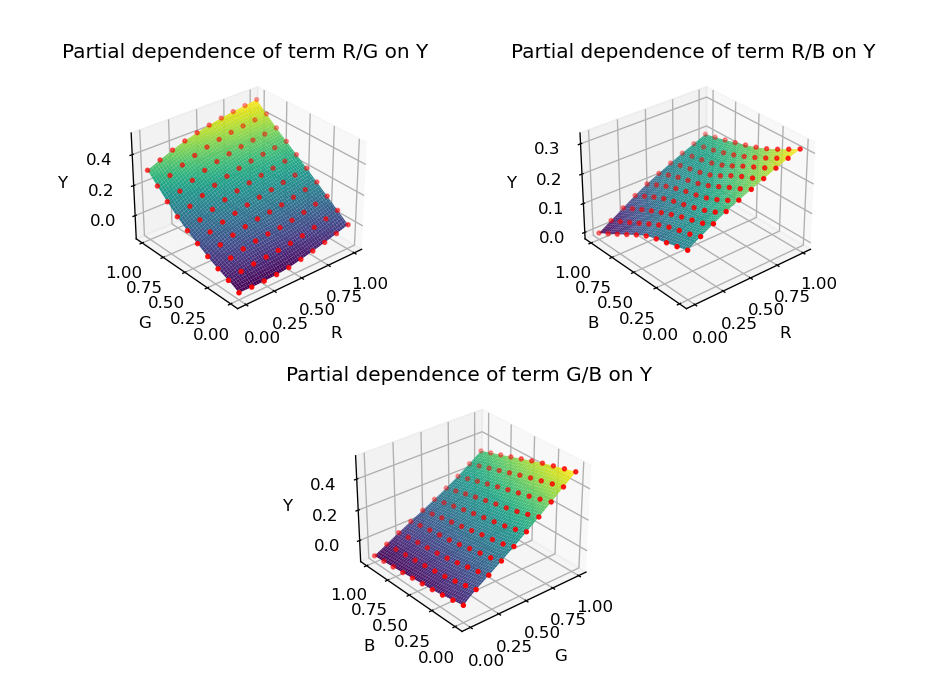
\includegraphics[width=\textwidth]{figures/partial.png}}{P-Spline predictors}
    \caption{Partial dependences on $Y$ with $\lambda = 0.1$ and 10 basis functions for Nikon D5100.}
    \label{fig:partialdep}
\end{figure}

Thus, our proposed model utilises distinct two-way interactions between the red, green, and blue channels transformed by third-order spline functions. The complexity of our model directly scales with the number of spline basis functions per feature:  for each of the three output channels, three tensor product features are used, resulting in total $3\times 3 \times n^2=9n^2$ terms. Models with 5, 10 and 20 have dimensionality of 225, 900 and 3600, respectively.

The model is simple to build, and many programming languages already offer the required building blocks, such as B-spline basis functions, and support matrix operations, such as tensor (Kroenecker) products and matrix multiplications. For example, one can use pyGAM \cite{serven2018pygam} in Python, mgcv \cite{wood2001mgcv}, or JOPSplus \cite{psplinesJoysPsplines} in R, or the Curve Fitting Toolbox \cite{MatlabCurveFitting2024} in MATLAB. The design matrix of basis functions is also efficient to compute via cardinal b-splines.
\chapter{Results}%
\label{ch:results}

% Add chapters similarly.

\chapter{Conclusions}
\label{ch:conclusion}

In this thesis we have presented a novel spline-based method for colour correction. The algorithm was built to extend the previous ideas in the literature, namely polynomial colour correction and its variants, as splines are also polynomials but are defined piecewise. The motive behind this research topic was, in general, to investigate the nature of colour transformations and to see if we can do better than the current algorithms that are simple in their design. They have performed well in practice, as seen by the continued use of a simple linear model for correction in the industry. However, expected advancements in display technology will likely lead to larger colour gamuts, necessitating more complex transformations. For example, in virtual and augmented reality (VR and AR) applications, errors in faithfully reproducing colours would likely result in loss of immersion for the user. 

A key contribution to this idea arises from the work of \citeauthor{finlayson2015color} in their publication on Root-Polynomial Colour Correction. In their paper, they stated, "From the low dimensional assumption of the reflectance spectra and a relatively good performance of the linear transform, we know that the mapping is approximately linear. Thus, we can expect that any non-linearities will be smooth across the sensor domain...". \cite[10]{finlayson2015color} 

Building on the insights, we took an approach of Penalized B-splines (P-splines), which enable the building of smooth yet non-linear models due to the ability to penalise the smoothness. To evaluate the performance of our model, we built a test bench in Python for colour correction algorithms since none exist, aside from the Colour Correction Toolbox \cite{fang2017colour} written in MATLAB, and it has not been maintained as of 2017. With the ever-growing adaptation of Python in the scientific community \cite{ozgur2017matlab}, we also wish to contribute and open-source our software for anyone.

The tests were conducted by generating synthetic response data for both the cameras and target human responses. This allowed us to experiment with various objects found in real life, such as skin tones, vegetation and human-made objects, collected from public datasets of hyperspectral images \cite{foster:2002}, \cite{Foster2022}, \cite{CAVE_0293}, \cite{wueller2009situ}. This allowed us to test the algorithms' real-life performance and the effect of training set size.

In this thesis, we sought to answer three research questions. First, we examined how our proposed algorithm fares against competitors, notably the PCC and RPCC models of different orders. We used the perceptual CIEDE2000 metric to assess the colour accuracy and observed that the proposed algorithms performed comparably to already established models despite not undergoing specialised optimisation. Furthermore, we did not notice a significant improvement in performance with the P-spline model using 20 spline basis functions rather than the P-spline model using five spline basis functions.

Our second research question concerned whether the training dataset and the camera spectral sensitivities affect the performance of colour correction algorithms. For this purpose, two datasets were chosen from different distributions and sizes. We picked Nikon D5100 and Sigma SD Merrill for the cameras. Both spectral sensitivities are publicly available and differ significantly due to colour sensing design \cite{D5100NPL}. For the Nikon, when trained on the larger dataset, we observed that all models but the neural network decreased in performance, even though the testing data set remained the same. Despite the decrease in performance, we also observed a change in the rank order of the models in favour of the P-spline models, which only slightly lost to the neural network. We observed the opposite for Sigma as the performance for P-spline models increased with the larger dataset. At the same time, it decreased in most cases for competitors other than the neural network.

A hypothesis for the varying performance across datasets and cameras is the shape of spectral sensitivities. For the Nikon, the transformation from RGB to XYZ is relatively simple, so a smaller but more evenly distributed dataset might be sufficient since the transformations are also bound to be more straightforward. In the case of Sigma, the transformation is naturally more complex due to the broad shape of spectral sensitivities, and a more extensive dataset might prevent overfitting.

It is also to be noted that while the combination of the Foster and Cave datasets contains more samples than the InSitu dataset, basic nearest neighbour downsampling was used to downscale the large hyperspectral images to a size more suitable for training. Despite this process, we found that there are still excessive amounts of near-duplicate samples, such as the black background in the images in figure \ref{fig:cave}. The authors from \cite{kucuk2023performance} utilised a more elegant method, where they first performed downsampling similarly but followed it by angular threshold filtering for removing similar samples. The InSitu dataset contains hand-picked reflectances from hyperspectral images taken purely for colour correction, and thus, the samples form an even distribution of real-life spectra.

In our third research question, we wanted to gain insight into the underlying transformation performed by our algorithm. This was accomplished by visually examining the partial dependencies and observing the exposure invariance as the penalty $\lambda$ varied. For the Nikon, the transformations were essentially linear, forming a hyperplane in three dimensions with a slight bend. On the contrary, the Sigma camera, as was also noticed in \cite{finlayson2015color}, requires a more aggressive colour correction. Thus, we saw more variation locally in the transformation than in the case of Nikon. As for the exposure invariance, we observed for both cameras that as we increase the penalisation $\lambda$, the models become more robust to changes in exposure. Intuitively, this makes sense as higher values of $\lambda$ drive the fits towards a linear one while lower value allows the fit to vary locally.

To conclude, we presented a novel spline-based model for colour correction that achieves a performance comparable to that of state-of-the-art methods. Our model is flexible in that by tuning a single parameter, $\lambda$, it can be used for cameras with varying spectral sensitivities. Regarding computational complexity, the largest model, with 20 spline basis functions, is similar to neural networks in the number of parameters (coefficients). Apart from the tensor products, our design matrix computation can be implemented efficiently through successive convolution of 0th-order B-splines. In addition, the models are very interpretable since they are linear in terms of their coefficients.

The P-spline models could be improved in numerous ways. Since the idea of P-splines is to employ a large number of basis functions at fixed knot intervals, for computational reasons, it would be wise to explore the usage of fewer basis functions instead but at custom locations and intervals. This is especially true for embedded implementations, where resources may be sparse. Further work could also explore optimising the P-spline models using a perceptual objective function, such as CIEDE2000, using a non-linear algorithm, such as BFGS. In this work, we used basic least-squares optimisation in the XYZ colour space, and as such, the results might not be optimal in the perceptual sense. Finally, more diverse and extensive datasets should be collected with more complex models, such as neural networks, which are becoming mainstream.

%%%%% Bibliography/references.

% Print the bibliography according to the information in ./tex/references.bib
% and the in-line citations used in the body of the thesis.
% \emergencystretch=2em
\printbibliography
%%%%% Appendices.
% Use only if it clarifies the structure of the document. Remember to
% introduce each appendix and its content.
\end{document}
